\documentclass[twoside,12pt,a4paper,catlan]{report}
%\includeonly{chapter04,list}

\usepackage[catalan]{babel}
\usepackage[utf8]{inputenc}
\usepackage{listings}
\usepackage[table]{xcolor}
\usepackage{tikz}
\usepackage{multicol}
\usepackage{hyperref}
\usepackage{array}
\usepackage{microtype}

\usepackage{fouriernc}
\usepackage[T1]{fontenc}


\usepackage{graphicx}
\usepackage{framed}
\usepackage{amssymb}
\usepackage{amsmath}

\usepackage{pifont}
\usepackage{ifthen}
\usepackage{makeidx}
\usepackage{enumitem}

\usepackage{titlesec}

\usepackage{fancyhdr}

\usepackage{skak}
\usepackage[scaled=0.95]{inconsolata}

\usepackage[dvipsnames]{xcolor}

\usetikzlibrary{patterns,snakes}
\pagestyle{plain}

\definecolor{keywords}{HTML}{44548A}
\definecolor{strings}{HTML}{00999A}
\definecolor{comments}{HTML}{990000}

\lstset{language=C++,frame=single,basicstyle=\ttfamily \small,showstringspaces=false,columns=flexible}
\lstset{
  literate={ö}{{\"o}}1
           {ä}{{\"a}}1
           {ü}{{\"u}}1
}
\lstset{xleftmargin=20pt,xrightmargin=5pt}
\lstset{aboveskip=12pt,belowskip=8pt}

\lstset{
    commentstyle=\color{comments},
    keywordstyle=\color{keywords},
    stringstyle=\color{strings}
}

\date{Draft \today}

\usepackage[a4paper,vmargin=30mm,hmargin=33mm,footskip=15mm]{geometry}

\title{\Huge Algorismes encarats a la programació competitiva, presents a la tecnologia i vida quotidiana}
\author{\Large Jan Matas Cantos}

\makeindex
\usepackage[totoc]{idxlayout}

%\titleformat{\subsubsection}
%{\normalfont\large\bfseries\sffamily}{\thesubsection}{1em}{}

\setcounter{secnumdepth}{3}
\setcounter{tocdepth}{3}

\begin{document}


%\selectlanguage{finnish}

%\setcounter{page}{1}
%\pagenumbering{roman}

\maketitle

%a) Motivació i interès pel tema.%
%b) Objectiu de la investigació.%
%c) Breu descripció de la metodologia emprada.%
%d) Resum dels resultats i conclusions%

%Cal evitar:%
%Utlitzar-lo per introduir el tema (per això tenim la introducció)%
%Redactar-lo a partir d’un copia i enganxa de la introducció o algunes parts de l’estudi.o Redactar-lo en futur: “aquest treball intentarà analitzar…”%
%Incloure frases d’abast general o ambigües “%
%Proporcionar moltes dades sense explicar-les.%
%Incorporar abreviatures, símbols o acrònims.%


\section{Resumen} 

Hoy en día, vivimos en una sociedad altamente digitalizada y en la cual la programación tiene una gran influencia. \newline

Partiendo del interés en el ámbito de la programación competitiva, los algoritmos y las matemáticas; se ha planteado estudiar e investigar si los algoritmos usados en la programación competitiva tienen algún uso en la tecnología o en la vida cotidiana. \newline

Después de una extensa exposición de los algoritmos más populares en la programación competitiva, se ha procedido a pensar y a buscar ejemplos de cómo estos algoritmos se aplican en la vida real, para afirmar o refutar la hipótesis. Asimismo, se han entrevistado dos personas con altos conocimientos algorítmicos. \newline

Finalmente, y en concordancia con las entrevistas, se ha podido comprobar que gran parte de los algoritmos de programación competitiva se emplean en la tecnología o en la vida cotidiana. Por otra parte, gracias a las entrevistas, se ha observado que tener un conocimiento algorítmico ayuda a entender mejor cómo funciona la tecnología en general, y que personas sin conocimiento algorítmico alguno, a veces, usan conceptos algorítmicos inconscientemente. \newline







\section{Abstract}

Nowadays, we live in a highly digitalised society which is largely impacted by programming. \newline 

Starting from the interest in the field of competitive programming, algorithms and mathematics; It has been proposed to study and investigate if the algorithms used in competitive programming have any use in technology, or in our daily lives.  \newline

After an extensive exposition of the most popular competitive programming algorithms, research has followed looking for examples on how these algorithms are applied in real life, checking to confirm or refute the hypothesis. In order to supplement this research work, and to gather additional views, a couple of highly skilled young programmers have been interviewed. \newline

Finally, and in alignment with the interviews outcome, the use of competitive programming algorithms in technology or in our daily lives has been successfully verified for the most part. On the other hand, and thanks to the interviews it has been observed that a better algorithmic knowledge helps understanding how digital technologies work. And likewise, that people without any algorithmic knowledge sometimes unconciously use key algorithmic concepts. \newline
\section{Agraïments}

En primer lloc, vull donar les gràcies a l'Alejandro Masana i al Javier Solà, ambdós tutors del meu treball de recerca, per tota l'ajuda, el seguiment i les idees que m'han proporcionat per la realització d'aquest treball. \newline

Estic molt agraït a l'Innokentiy Kaurov i al Sergio Dominguez, tots dos joves programadors amb altíssims coneixements d'algorísmia, per haver dedicat una part del seu temps a respondre molt amablement les meves preguntes. \newline

També estic molt agraït a l'Omer Giménez, programador a \emph{Google}, per haver resolt tots els dubtes que tenia relacionats amb \emph{LaTeX} (l'eina emprada en aquest treball) i per educar-me a mi i a molts altres joves en l'algorísmia. \newline

Finalment, vull agrair igualment el suport dels meus amics i família, en especial el del meu pare, per donar-me la seva opinió amb el treball i fer crítiques constructives. \newline

Sense ells aquest treball no hauria sigut possible. A tots ells moltes gràcies.



\tableofcontents

\include{preface}

\pagenumbering{arabic}
\setcounter{page}{7}

\newcommand{\key}[1] {\textbf{#1}}

% index
\include{introducció}
\section{Motivació pel tema}

Fa un parell d'anys, tot passant l'estona veient vídeos a YouTube, l'aplicació em va recomanar un curt on es presentaven breument els millors llenguatges de programació actuals. De seguida va captar la meva atenció i vaig voler saber-ne més. Vaig cercar un vídeo del llenguatge de programació \emph{Python} i em vaig anar enganxant. Em vaig insta\lgem ar el llenguatge de programació a l'ordinador i vaig començar a aprendre a programar de forma autodidàctica. \newline

Un any més tard, el meu cosí gran em va introduir en el món de la programació competitiva, em va parlar de la web \emph{Jutgel.org} i de tot de recursos en línia disponibles al meu abast. A partir d'aquí em vaig llançar a la programació competitiva, aprenent els seus algorismes lògics i matemàtics, resolent problemes a casa i participant en competicions tant en línia com de manera presencial. \newline

A l'hora de fer el Treball de Recerca, tant la família a casa, com els professors a l'escola, em van recomanar fermament que triés un tema que m'agradés i motivés. \newline

Inicialment, vaig pensar a fer el treball enfocat a la programació i el desenvolupament web. Més endavant, el meu interès per la programació competitiva va fer que em decantés a triar un tema que hi estigués relacionat. \newline

Realment aquest és un tema que m'apassiona i motiva molt pel fet que combina les matemàtiques, la programació i el pensament lògic.  



%El tema em motiva tant pel fet que m'encanten les matemàtiques, la programació i encara més resoldre problemes utilitzant la lògica, els algorismes i el pensament.%

%Com que a casa ja aprenc pel meu compte tots aquests algorismes i resolc problemes diversos de programació doncs vaig pensar que si feia el treball de recerca d'un tema relacionat amb tot allò que gaudeixo tant fer, aquest passaria de ser un treball pesat i avorrit a una feina que m'agrada i gaudeixo fent.%


%a causa del treball i l'esforç que comporta realitzar aquest, jo he seguit el consell i finalment he trobat un tema que m'apassiona com són els algorismes encarats a la programació competitiva.%
\include{hipòtesi}

\part{Marc Teòric}
\chapter{Algorismes}
\section{Què és un algorisme?}


Un algorisme és un conjunt de regles definides que permet solucionar un problema d'una determinada manera de forma inequívoca mitjançant operacions sistemàtiques i finites. Aquestes instruccions, definides i ordenades en funció de les dades, resolen un problema o tasca. \newline

La paraula "algorisme" avui dia l'associem a la tecnologia, però, realment aquest concepte té segles d'antiguitat, de fet, s'aproxima que el seu origen etimològic prové del matemàtic de l'edat mitjana, al-Jwārizmī. El que sí que està clar és que exemples d'algorismes són les operacions bàsiques de les matemàtiques: la suma, la resta, la multiplicació i la divisió. I aquestes operacions fa molt de temps que s'utilitzen. \newline

Cal recalcar que un algorisme no té per què estar relacionat amb la matemàtica o la tecnologia sinó que un tipus d'algorisme pot ser simplement una recepta de cuina o un full d'instruccions per muntar un moble d'IKEA.
\section{Característiques}

\begin{itemize}
\item Les instruccions i regles de cada algorisme són finites, és a dir, hi ha un nombre determinat d'elles.
    \item En general són passos elementals i simples però molt nombrosos.
    \item Les instruccions s'apliquen de forma ordenada.
    \item Sempre que un algorisme estigui ben implementat, aquest tindrà un resultat final.
    \item Davant les mateixes dades/input, el resultat final sempre serà exactament igual, per exemple la suma d'1 + 1 sempre dona com a resultat 2.
\end{itemize}
\section{Parts}

\begin{itemize}
\item L'entrada/input: són les dades sobre les quals s'apliquen les instruccions de l'algorisme. En el cas que busquéssim "casa" a Google, l'input seria "casa".
\item Realització de les instruccions que duu a terme l'algorisme. En l'exemple anterior, aquest procés és invisible, però bàsicament l'algorisme de Google busca les WEBS més populars les quals el seu domini (nom) coincideixin amb l'input donat per l'usuari.
\item La sortida/output: és el resultat de l'algorisme. En l'exemple anterior, Google ens mostraria per pantalla les WEBS més populars les quals el seu domini (nom) coincideixin amb l'input donat per l'usuari. En el cas d'una recepta d'un pastís, l'output seria el pastís en si.
\end{itemize}

\section{Utilitats}

Un algorisme, com hem dit anteriorment ens ajuda a resoldre un problema de forma sistemàtica i inequívoca, per exemple, cada vegada que hem de posar la rentadora, simplement introduint-hi la roba i una mica de detergent i suavitzant ja ens deixà la roba neta, l'algorisme de la rentadora s'encarrega de tot. \newline

Tot i això, amb l'arribada de la tecnologia i els ordinadors, els algorismes cobren encara més importància, ja que ens permeten obtenir un resultat a partir d'un input de dades immens en qüestió de mi\lgem isegons, en concret, un ordinador quotidià pot realitzar unes 4e8 operacions per segon. \newline

Per exemple dels milions de vídeos que existeixen a YouTube, aquest gràcies a l'algorisme s'encarrega d'escollir i mostrar-nos els que creu que ens seran del nostre gust. \newline

En definitiva els algorismes tenen moltes utilitats i ens ajuden molt, durant el transcurs d'aquest treball en veurem alguns conjuntament amb les seves utilitats específiques.
\section{Algorismes presents a Internet}


Algun cop t'has adonat que Netflix et recomana pe\lgem ícules/sèries del teu gust i de l'estil de les vistes anteriorment?, o que Google et mostra anuncis de quelcom que has estat interessat recentment en les teves cerques, exemples d'aquests n'hi ha molts, però tots tenen quelcom en comú: \textbf{funcionen gràcies a un algorisme de recomanació}, bàsicament com que Google té les dades de l'usuari (el que busca, compra a Internet) doncs mitjançant l'algorisme saben el que ens agrada i per tant ens recomanen coses del nostre gust.
\section{Complexitat d'Un Algorisme (Big O Notation)}

Abans de veure els alguns dels algorismes aplicats a la programació que existeixen hem d'entendre bé el que és Big O Notation.
Quan parlem de rendiment i optimització, és important tenir una regla per determinar que tan bo o que tan dolent és un algorisme, per això existeix Big O Notation que ens descriu el pitjor escenari, és a dir, el màxim en la quantitat més gran de repeticions que l'algorisme ha d'executar. \newline

Big O Notation és utilitzat a les ciències computacionals per descriure la complexitat i el rendiment d'un algorisme, un factor que hem de tenir en compte és que la majoria d'algorismes canvien el seu rendiment depenent de la quantitat d'input que ha de processar, és a dir alguns algorismes funcionen amb un bon rendiment quan la quantitat de l'input és petit, però perden efectivitat quan incrementes l'input.
Generalment, Big O Notation descriu el pitjor escenari possible, és a dir, el màxim nombre de repeticions que l'algorisme ha d'executar. \newline \newline

\begin{description}

\item[$O(1)$]
\index{algorisme de temps constant}

Aquesta expressió indica temps constant, el que significa és que l'algorisme s'executarà amb el mateix rendiment sense importar la mida de l'input, és a dir, no es veurà afectat per la quantitat de dades que estiguem manejant.
Aquesta notació és la més eficient, òptima i amb el millor rendiment. \newline

\underline{Exemple:} \newline

\begin{lstlisting}
int a = 5;
int b = 10;
int c = a + b;
cout << c << endl; // 15
\end{lstlisting}

\newpage

\item[$O(\log n)$]
\index{algorisme logarítmic}
Aquesta expressió índica que el temps augmenta linealment, mentre que $n$ augmenta exponencialment, per tant, si es triga 1 segon a processar 10 elements, en conseqüència es trigaran 2 segons per calcular-ne 100, 3 per 1000 i així successivament. \newline

\underline{Exemple:} \newline

\begin{lstlisting}
int n;
cin >> n; // Input -> 512

while (n > 1){
    cout << n << " ";
    n = n / 2;
}

// Output -> 512 256 128 64 32 16 8 4 2
\end{lstlisting}

En aquest cas, n = 512, però el programa només es repeteix $\log_{2}(512)$ vegades, és a dir, 9 vegades, ja que a cada pas, dividim $\frac{n}{2}$ . \newline

\item[$O(n)$]
\index{algorisme lineal}

Aquesta expressió indica un creixement lineal, la complexitat de l'algoritme augmenta de manera proporcional a la dimensió de l'input.
Aquesta notació és bastant eficient, i té un molt bon rendiment. \newline

\underline{Exemple:} \newline

\begin{lstlisting}
int n;
cin >> n; // Input -> 8 (per exemple)

for (int i = 1; i <= n; i++){
    cout << i << " " << endl;
}

// Output -> 1 2 3 4 5 6 7 8

\end{lstlisting}

En aquest exemple, el nostre programa ens escriu tots els nombres d'1 fins $n$ i, per tant, s'ha de repetir $n$ vegades. \newpage

\item[$O(n \log n)$]

Aquesta expressió és una fusió de $O(n)$ i de $O(\log n)$.
Es diu que un algorisme té una complexitat temporal quasi lineal $O(n \log n)$ quan cada operació de les dades d'entrada té una complexitat temporal de $O(\log n)$ o quan l'algorisme ordena tota l'entrada i, per tant, és $O(n \log n)$, ja que és el cost de qualsevol algorisme d'ordenació eficient (merge sort, etc.) \newline

\underline{Exemple:} \newline

\begin{lstlisting}
int n;
cin >> n; // Input -> 4

vector llista;
for (int i = n; i >= 1; i--){
    llista.push_back(i);
}

// llista [4, 3, 2, 1]
sort(llista.begin(), llista.end());
// llista [1, 2, 3, 4]

\end{lstlisting}

\item[$O(n^2)$]
\index{algorisme quadràtic}

Aquesta expressió indica que el creixement en complexitat és directament proporcional al quadrat de la mida de l'input.
Aquest algoritme és poc eficient quan l'input és gran i, per tant, és molt poc recomanable. \newline

\underline{Exemple:} \newline

\begin{lstlisting}
int n;
cin >> n; // Input -> 3

for (int i=1; i<=n; i++){
    for (int j=1; j<=n; j++){
        cout << i << " " << j << " ";
    }
}

// Output -> 1 1  1 2  1 3  2 1  2 2  2 3  3 1  3 2  3 3
\end{lstlisting}
\newpage

Cal dir que la complexitat temporal és tan sols una aproximació, per exemple, si un algorisme treballa específicament en temps $O(n + n^2)$, direm simplement que funciona en $O(n^2)$, ja que la suma de $n$ és irrellevant amb el $n^2$ . \newline

\end{description}

\begin{center}
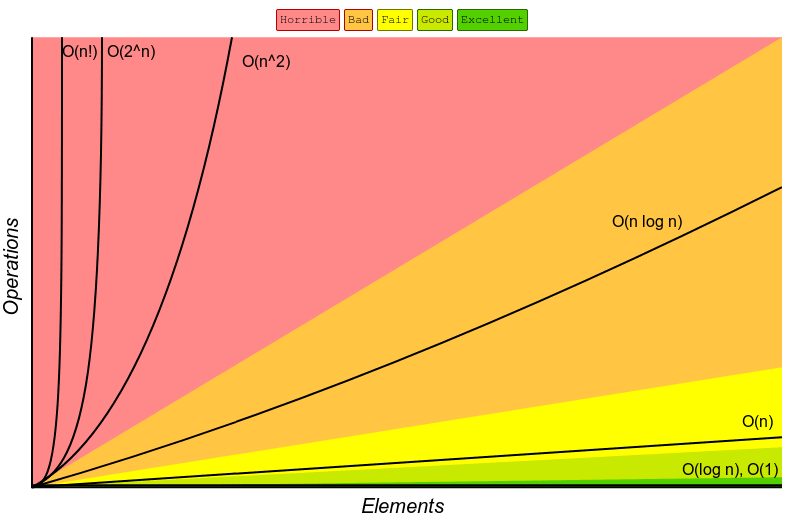
\includegraphics[width=.9\textwidth]{compl.png}

\caption{\emph{Figura 1: Operacions-Temps. Font: \url{https://towardsdatascience.com/understanding-time-complexity-with-python-examples-2bda6e8158a7}}}
\end{center}

A la Figura 1 podem observar la relació Temps-Operacions de les complexitats de $n$ més típiques en la programació, bàsicament el gràfic ens indica el rendiment i l'eficiència de cada complexitat. \newline




\section{Algorismes De Programació Competitiva}
\subsection{Tipus d'algorismes}

Els algorismes de programació competitiva es classifiquen bàsicament en dues variants:

\begin{itemize}
    \item Algorismes Iteratius
    \item Algorismes Recursius
\end{itemize}

Entendre aquestes dues variants és molt important puix que facilita l'enteniment de què veurem més endavant com la programació dinàmica, DFS, BFS, entre altres (és totalment normal que costi d'entendre i que necessitis llegir les explicacions diverses vegades per comprendre la recursió). \newline

Sovint els problemes es poden resoldre amb les dues tècniques (recursió i iteració) però depenent de la situació, preferirem fer servir una o l'altra. \newline
\include{Iteració}
\subsubsection{Recursius}

La recursió és una tècnica la qual empra una funció recursiva, aquesta funció consta de dues parts:

\begin{itemize}
\item Cas base -> finalitza la recursió.
\item Cas recursiu -> continua la recursió (crida la funció recursiva).
\end{itemize}

La recursió ens l'hem d'imaginar com un arbre en el qual cada crida recursiva forma una nova branca d'aquest i s'allarga fins que arriba a un cas base. \newline

De nou, posaré l'exemple de la seqüència de Fibonacci per comparar la recursió amb la iteració. \newline

La formula a utilitzar és la mateixa que la que hem utilitzat en la recursió. \newline

fib_n =
\begin{cases}
0 & \text{si $n = 0$}\\
1 & \text{si $n = 1$}\\
fib_{n-1}+fib_{n-2}& \text{si $n \geq 2$}
\end{cases} \newline \newline

Els primers dos casos: $n = 0$ i $n = 1$, seran els casos base. \newline

L'últim cas: $n \geq 2$, serà el cas recursiu. \newline

Donada qualsevol $n$ tal que la $n-esima$ posició en la seqüència de Fibonacci, amb l'ús de la recursió podem trobar $fib_n$ amb una complexitat de $O(2^n)$.

Cal recalcar que podem fer-ho també amb una complexitat de $O(n)$, però requereix l'ús de la programació dinàmica. \newline

\begin{lstlisting}
int fib(int n){

    if (n == 0) // primer cas base
        return 0;

    if (n == 1) // segon cas base
        return 1;

    return fib(n - 1) + fib(n - 2); // cas recursiu
}

int main(){
    cout << "Introdueix n: " << endl;
    int n; // Input -> 9
    cin >> n;
    cout << fib(n); // Output -> 34
}
\end{lstlisting}


\begin{center}
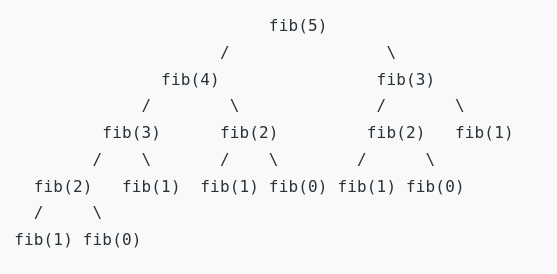
\includegraphics[width=.9 \textwidth]{crides.png}

\caption{\emph{Figura 3: Crides recursives fibonacci. Font: \url{https://www.geeksforgeeks.org/program-for-nth-fibonacci-number/}}}
\end{center}

A la figura 3, podem analitzar totes les crides recursives que es realitzen amb $n = 5$.

Podem observar que hi ha crides repetides i que es poden optimitzar per no haver de recalcular-les de forma estúpida, aquestes optimitzacions es poden dur a terme com he dit anteriorment, amb la programació dinàmica. \newline

A la figura 3, considerem que la branca de fib(3) i fib(2) està repetida.
\subsection{Força Bruta}

Aquests algorismes són exactament el que sonen, mètodes senzills per resoldre un problema, provant totes les possibles possibilitats d'aquest fins a trobar la solució bona.

Per exemple, si tenim un cadenat de tres dígits entre 0 i 9 i ens oblidem de la contrasenya, com que no volem comprar un altre cadenat i no podem recordar cap dígit de la contrasenya, haurem d'utilitzar un mètode de força bruta per endevinar la contrasenya, és a dir, haurem de provar totes les possibilitats (0,0,0 / 0,0,1 / 0,0,2 / etc.), en el pitjor dels casos ens caldrien $10^3$ o 1000 intents, ja que tenim 3 dígits i per cada dígit hi ha 10 números diferents com a possibilitats, si tinguéssim un cadenat de 4 dígits, ara el nombre d'intents en el pitjor cas per trobar la contrasenya passaria a ser $10^4$ o 10000 intents .

Un exemple clàssic en informàtica és el problema del venedor ambulant (TSP). Suposem que un venedor ha de visitar 10 ciutats del país. Com es determina l'ordre en què s'han de visitar aquestes ciutats de manera que es minimitzi la distància total recorreguda?
La solució de força bruta és simplement calcular la distància total per a cada ruta possible i després seleccionar la més curta. Això no és especialment eficient perquè és possible eliminar moltes rutes possibles mitjançant algorismes inte\lgem igents, en canvi, la força bruta prova totes les opcions.

La complexitat temporal de la següent força bruta és $O(n \cdot m)$. Per tant, si cerquéssim una cadena de $n$ caràcters en una cadena de $m$ números mitjançant la força bruta, ens caldria $n \cdot m$ intents.

En la següent imatge veurem un algorisme de força bruta molt simple que endevina el codi d'un cadenat de 4 dígits. \newline

\begin{lstlisting}
void endivinarCodi(int contrasenya){
    for (int i = 0; i < 10000; i++){
        if (i == contrasenya){
        cout << "L'algorisme ha endevinat el teu codi!"<< endl;
        cout << "La contrasenya es: " << i << endl;
        }
    }
}

int main(){
    int contrasenya;
    cout << "Introdueix un codi, entre 0000 i 9999:" << endl;
    cin >> contrasenya;
    endivinarCodi(contrasenya);
}
\end{lstlisting}

\newpage

L'anterior codi el que fa és demanar un codi a l'usuari i després va provant dels números 0000 al 9999 i mira si coincideixen amb el codi donat.

És a\lgem ucinant la velocitat a la qual l'ordinador endevina el codi, és per això que és molt important tenir codis llargs i amb dígits diversos, puix que els $hackers$ utilitzen un l'algorisme de força bruta una mica modificat per endevinar els codis. \newline

\begin{center}
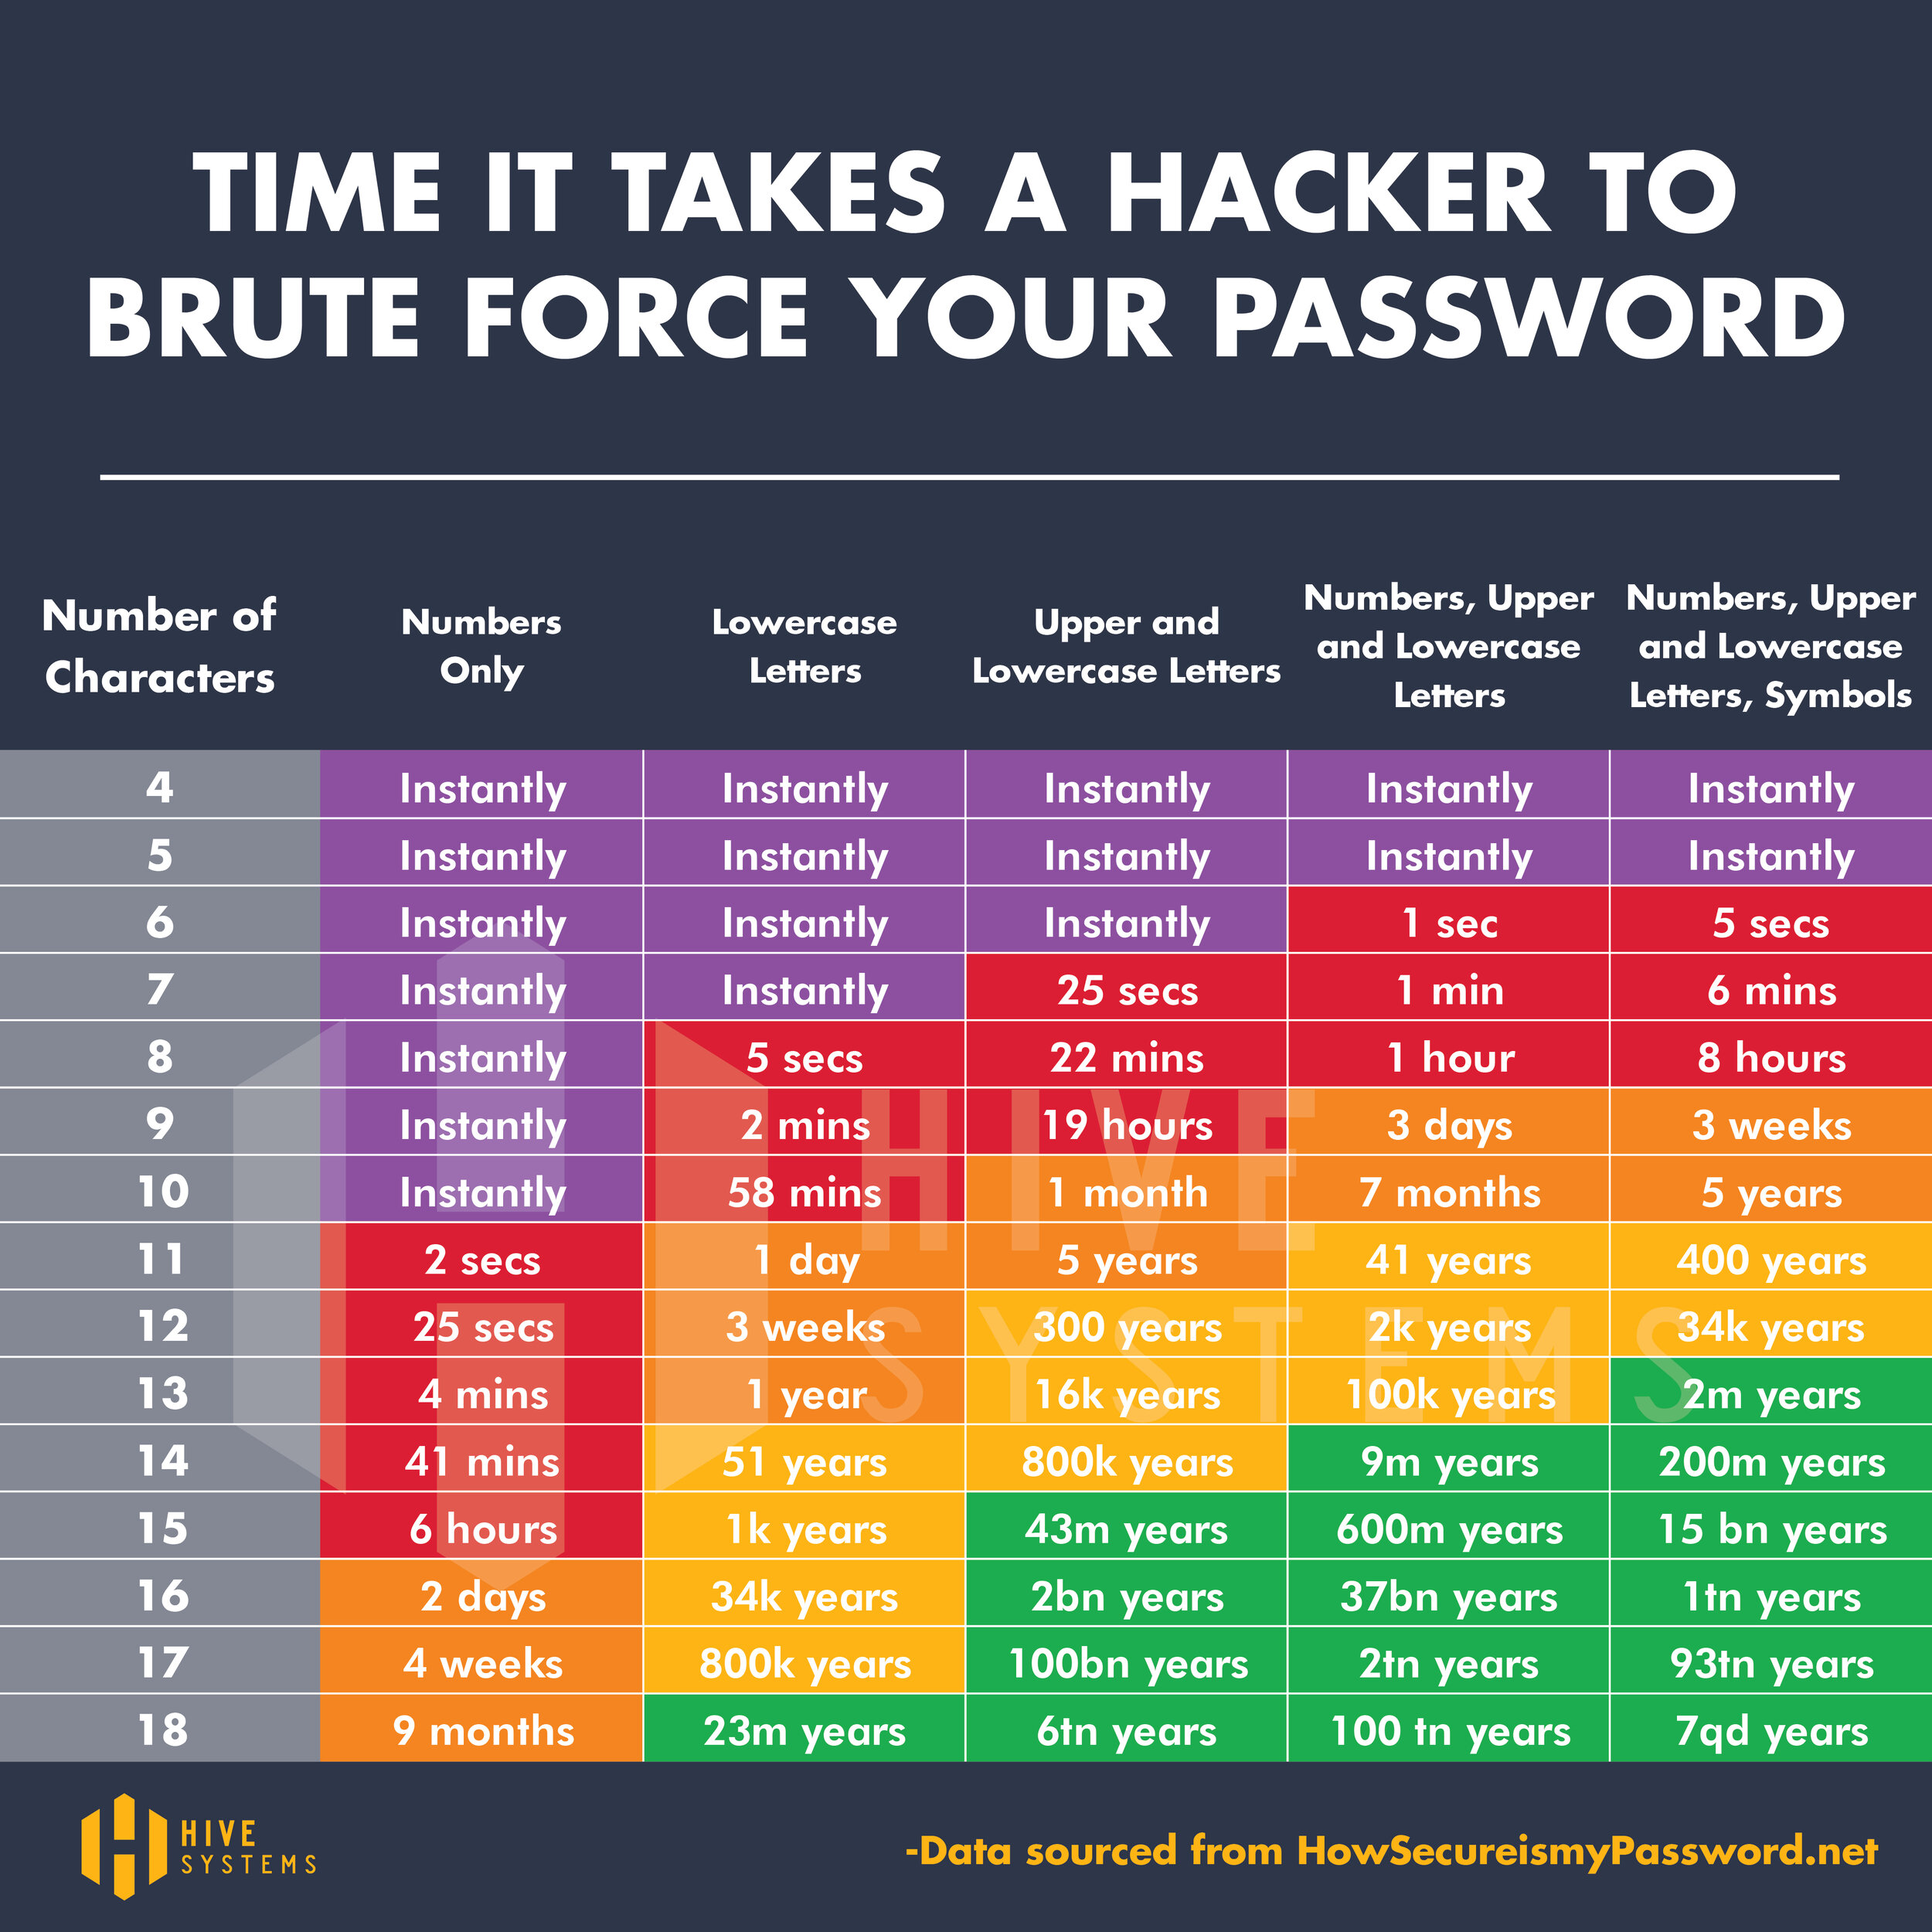
\includegraphics[width=.7 \textwidth]{time_hackers.jpg}

\caption{\emph{Figura 4: Temps en el qual els $hackers$ endevinen les contrasenyes mitjançant la força bruta.}}
\end{center}
\subsection{Greedy}

El conegut i molt popular algorisme $Greedy$, és un algorisme que construeix una solució peça per peça, sempre escollint la peça que ens dona el benefici més evident i immediat. \newline
 
Imagineu que aneu a fer senderisme i que el vostre objectiu és arribar al cim més alt possible. Ja teniu el mapa abans de començar, però hi ha milers de camins possibles que es mostren al mapa. Ets massa mandrós i simplement no tens temps per avaluar-los. \newline

Comença a caminar amb una estratègia senzilla: agafar els camins que sembli que ens portaran més amunt, per tant, només cal agafar els camins que tenen més pendent. Sembla una bona estratègia per fer senderisme. Però és sempre el millor? \newline

Un cop acabat el viatge i tot el teu cos està adolorit i cansat, mires el mapa de senderisme per primera vegada. Oh Déu meu! Hi ha un riu fangós que hauria d'haver creuat, en lloc de continuar caminant cap amunt. Això vol dir que un algorisme $Greedy$ tria la millor opció immediata i mai reconsidera les seves eleccions. Pel que fa a l'optimització d'una solució, això simplement vol dir que la solució $Greedy$ intenta trobar solucions òptimes locals, que poden ser moltes, i es pot perdre una solució òptima global.\newline

Per això un algorisme $Greedy$ no és sempre efectiu, ja que encara que sempre triï el millor camí en cada decisió, potser, per agafar el millor camí total, primer havies d'agafar un camí aparentment dolent per després seguir amb camins més òptims i que portin a una solució global més favorable. \newline

Un exemple d'estratègia $Greedy$ a la vida real és la següent: imaginem que els nostres pares ens han donat 10 euros per comprar el que vulguem en una botiga de roba, com que volem aprofitar els diners que ens han donat, volem gastar el major nombre d'euros possibles, per tant, la nostra estratègia $Greedy$ podria consistir a mirar tots els productes ordenats de més cars a més barats i comprar cada producte si ens el podem permetre. \newline

Tot i així, aquesta estratègia és sempre òptima?

La realitat és que no, en alguns casos, per maximitzar la despesa, és millor comprar molts productes barats que no pas algun de car, per entendre-ho millor mirem els següents exemples: 


\begin{itemize}

\item Posem que els preus dels productes fossin els següents [2, 3, 3, 8] i que tenim un total de 10 euros, en aquest cas la nostra estratègia $Greedy$ funcionaria, ja que primer compraríem el producte de 8 euros i després el de 2 euros.

\item Posem que els preus dels productes fossin els següents [3, 3, 4, 9] i que tenim un total de 10 euros, en aquest cas la nostra estratègia $Greedy$ no funcionaria, puix que primerament compraríem el producte de 9 euros, en conseqüència ens quedaria 1 euro i no podríem comprar cap producte més, tot i així, en aquest cas, la compra òptima, seria obtenir els dos productes de 3 euros i el de 4 euros, en total ens gastaríem els 10 euros.

\end{itemize}

Seguidament, trobem la implementació de l'estratègia $Greedy$ comentada anteriorment.



\begin{lstlisting}
int nombreProductes; cin >> nombreProductes;

int dinersTotals; cin >> dinersTotals;

vector<int> preuProductes(nombreProductes);

for (int i = 0; i < nombreProductes; i++){
    cin >> preuProductes[i];
}

sort(preuProductes.rbegin(), preuProductes.rend());
// ordenem els preus de més car a més barat

int dinersGastats = 0;

for (int i = 0; i < nombreProductes; i++){
    if (dinersTotals >= preuProductes[i]){
        // si ens podem permetre el producte,
        // el comprem
        dinersGastats += preuProductes[i];
    }
}


cout << dinersTotals - dinersGastats << endl;
// dinersTotals - dinersGastats = 
// diners que ens han quedat 
\end{lstlisting}




\subsection{Divideix i venceràs}

Aquest algorisme com bé ens indica el seu nom es basa a dividir les dades per poder tractar-les amb més facilitat i consta de 3 parts essencials: \newline

Dividir: Descompondre el problema en subproblemes del mateix tipus. Aquest pas involucra descompondre el problema original en petits subproblemes. Cada subproblema ha de representar una part del problema original. En general, aquest pas empra un enfocament recursiu per dividir el problema fins que no és possible crear un subproblema més. \newline

Vèncer: Resoldre els subproblemes recursivament. Aquest pas rep un gran conjunt de subproblemes a ser resolts. Generalment, a aquest nivell, els problemes es resolen per ells mateixos. \newline

Combinar: Combinar les respostes apropiadament. Quan els subproblemes són resolts, aquesta fase els combina recursivament fins que aquests formen la solució al problema original. Aquest enfocament algorítmic treballa recursivament i els passos de conquesta i fusió treballen alhora i, per tant, pot semblar que es faci en un sol pas. \newline

Aquest mètode és molt útil, puix que usualment ens ajuda a reduir la complexitat de l'algorisme a fer ús, per exemple podem ordenar una llista amb l'algorisme $Bubble Sort$ que té una complexitat de $O(n^2)$, però amb $Merge Sort$ (algorisme de divideix i venceràs) podem reduir la complexitat a $O(n log n)$.
\subsubsection{Cerca Binària}

La cerca binària és un algorisme eficient per trobar un element d'una llista ordenada d'elements.

Funciona dividint repetidament per la meitat la part de la llista que podria contenir l'element, fins que hàgiu reduït les ubicacions possibles a només una i llavors voldrà dir que hem trobat l'element que buscàvem.

\newline
La complexitat de la cerca binària és de $O(log n)$.

Inconscientment, quan juguem al joc d'endevinar un número de l'1 al 100, si juguem a la perfecció (provant el número meitat de l'interval), estem utilitzant la cerca binària, ja que a cada intent, com que ens diuen si el número que hem provat és més gran o més petit que el número que ha pensat, doncs, reduïm els números a la meitat, també podem assegurar que, si el número es troba entre l'interval d'1 i 100 l'endevinarem en un màxim de 7 intents, ja que $\log_{2}(100)$ = 6.6438... i, per tant, l'arrodonim a un màxim de 7 intents. \newline

En canvi, si provéssim els números des de l'1 fins al 100 (1,2,3,4,5...) seria una forma molt poc eficient, ja que en el pitjor dels casos necessitaríem 100 intents i, per tant, seria $O(n)$ (Força bruta), en canvi, si provem els nombres meitat de l'interval, necessitarem $\log_{2}(100)$ intents i, per tant, serà $O(log n)$ (Cerca binària) on $n$ és el nombre màxim que pot ser el nombre secret (en aquest cas 100). \newline

En la següent imatge podem observar l'algorisme de cerca binària aplicat a aquest joc, és un programa interactiu, és a dir, es demana un número secret a l'usuari i seguidament l'algorisme prova el número meitat entre el 0 i el 100 (en aquest cas 50), llavors l'usuari ha d'introduir si el nombre (50) és igual, major o menor al nombre secret, en cas que sigui major, l'algorisme descarta l'interval 0-50, en canvi, si és menor, l'algorisme descarta l'interval 50-100, en el següent intent, el programa prova amb un número que estigui a la meitat del nou interval, i així successivament fins que encerta el número.

\newpage

\begin{lstlisting}
void Endevina_Nombre(){
    int meitat, intents = 0, esquerra = 1, dreta = 100;
    char resposta;
    // Aquí comença la cerca binària
    while (dreta > esquerra + 1){
        intents += 1;
        meitat = (esquerra + dreta) / 2;
        cout << "L'algorisme ha provat el numero: " << meitat << endl;
        cin >> resposta;
        if (resposta == '='){
            cout << "Nombre secret: " << meitat << endl;
            cout << "Intents: " << intents << endl;
            break;
        }
    } 
    else if (resposta == '>')
        dreta = meitat;
        
    else if (resposta == '<')
    esquerra = meitat;
}

// Input -> > < > > > =
// Output -> L'algorisme ha provat el número: 50
// L'algorisme ha provat el número: 75
// L'algorisme ha provat el número: 62
// L'algorisme ha provat el número: 68
// L'algorisme ha provat el número: 71
// L'algorisme ha provat el número: 73
// Nombre secret: 73
// Intents: 6
}
\end{lstlisting}
%\include{itrec}%
\subsection{Programació Dinàmica}

La programació dinàmica és principalment una optimització de la recursivitat simple i la força bruta (brute force). La idea principal de la programació dinàmica és dividir el problema sencer en petits subproblemes i emmagatzemar les solucions d'aquests de manera que més endavant quan sigui necessari, no els hàgem de tornar a recalcular. \newline

La programació dinàmica és un algorisme importantíssim en la programació competitiva, ja que és aplicable a molts problemes i és molt útil per tant ens convé aprendre a fer-la servir. \newline

Aquesta optimització ens redueix molt la complexitat temporal de l'algoritme, sovint passa de $(2^n)$, complexitat exponencial a $O(n)$, complexitat lineal. \newline

Un exemple de problema molt típic de programació dinàmica és el següent:

Calcula el nombre de maneres de construir una suma $n$ tirant un dau una o més vegades, el dau és un dau de valors [1,2,3,4,5,6].

Per exemple, si $n = 3$, hi ha 4 maneres diferents.

\begin{itemize}
\item 1 + 1 + 1
\item 1 + 2
\item 2 + 1
\item 3
\end{itemize}

En el següent codi podem apreciar el codi que resol aquest problema amb programació dinàmica. \newpage

\begin{lstlisting}
int n; cin >> n; // Input -> 3

vector dp(n+1);
dp[1] = 1;
for (int i=2; i<=n; i++){
    dp[i] += dp[i-1];
    dp[i] += dp[i-2];
    
    if (i >= 3)
        dp[i] += dp[i-3];
        
    if (i >= 4)
        dp[i] += dp[i-4];
        
    if (i >= 5)
        dp[i] += dp[i-5];
        
    if (i >= 6)
        dp[i] += dp[i-6];
}

cout << dp[n] << endl; // Output -> 4
\end{lstlisting}

El que fem en el codi és dividir el problema en $n$ parts, i per a cada número de 2 a $n$, li sumem el nombre de combinacions del nombre en el qual estem menys els números que podem arribar fins a aquell nombre [1,2,3,4,5,6], tot i així, per exemple al nombre 3 no li podem sumar el nombre de combinacions de:

\begin{itemize}
\item 3 - 4
\item 3 - 5
\item 3 - 6
\end{itemize}

Això és degut al fet que en cap moment tenim valors negatius en les tirades, finalment a $dp[n]$, tenim el nombre total de combinacions per a qualsevol $n$. \newline \newline

Un altre exemple de l'ús de la programació dinàmica una mica més difícil comparat amb el que hem vist anteriorment, és el següent: donats dos enters n i m i un tauler amb n files i m columnes plens de "." (llocs per on podem passar) i "X" (trampes per on no podem passar) hem de contar el nombre de camins diferents que van des de la cantonada inferior dreta fins a la cantonada superior esquerra.

Primer llegirem el taulell i l'emmagatzemem en un vector 2d (mapa), ja que hi ha files i columnes, seguidament crearem un vector 2d també (dp) on emmagatzemarem a cada posició i, j (x, y) del mapa el nombre de camins possibles per arribar a aquesta posició $i, j$ $(x, y)$.

Seguint aquesta regla, dp[1][1] haurà de ser igual a 1, ja que per arribar a la posició inicial només tenim un camí possible i dp[n][m] haurà de ser igual a la resposta final, ja que és el nombre de camins per arribar fins a la cantonada superior esquerra.

Per trobar els camins primer iterarem per tot el mapa amb un doble bucle for i si en la posició $i, j$ $(x, y)$ del mapa no hi ha una trampa, farem la següent operació: \newline

$dp[i][j]$ \hspace{0.1cm} = \hspace{0.1cm} $dp[i-1][j]$ \hspace{0.1cm} + \hspace{0.1cm} $dp[i][j-1]$ \newline

Aquesta fórmula la podem deduir perquè el nombre de camins de qualsevol posició $i, j$ (menys quan $i = 1$ o quan $j = 1$) és igual a la suma del nombre de camins de la posició $i-1,j$ $+$ $i,j-1$, això és a causa del fet que per arribar a qualsevol posició $i,j$, les úniques coordenades de les quals podem venir són $i-1,j$ i $i,j-1$.
Finalment, simplement retornarem dp[n][m].

En el següent codi observem una part de la implementació per resoldre aquest problema amb programació dinàmica.

\begin{lstlisting}
int n,m; cin >> n >> m; // Input -> 3 8

vector<vector> dp(n+1, vector(m+1));
dp[1][1] = 1;

vector<vector> mapa(n+1, vector(m+1));
// Input -> .......X
//           .X.X.X..
//           X.......

for (int i=1; i<=n; i++){
    for (int j=1; j<=m; j++){
        cin >> mapa[i][j];
        if (mapa[i][j] == 'X') 
            // hem trobat una trampa 
            per tant no fem res
            continue; 
    
        if (i == 1 && j > 1)
            dp[i][j] = dp[i][j-1];
            
        else if (j == 1 && i > 1)
            dp[i][j] = dp[i-1][j];
            
        else if (i > 1 && j > 1)
            dp[i][j] = dp[i-1][j] + dp[i][j-1];
    }
}

cout << dp[n][m] << endl; // Output -> 4
\end{lstlisting}

En aquest cas no hi han gaires camins possibles gràcies al fet que hi ha moltes trampes, però si no n'hi hagués tantes i el tauler fos més gran podríem veure que el nombre de camins augmenta exponencialment.


\subsection{Backtracking}

El backtracking és un algorisme que resol els problemes de forma recursiva considerant totes les combinacions possibles per resoldre un problema i que construeix la solució de manera ascendent, una peça a cada torn, també descarta totes aquelles solucions que no satisfan les limitacions del problema en qualsevol moment.

S'utilitza el backtracking en els següents problemes:

\begin{itemize}
    \item Problema de decisió -> Es busca una solució factible.
    \item Problema d'optimització -> Es busca una solució òptima
    \item Problema d'enumeració -> Es busquen totes les solucions factibles.
\end{itemize}

Tot i això, la majoria de problemes que es resolen amb backtracking també es poden resoldre amb altres algorismes com greedy o programació dinàmica amb una complexitat temporal $O(log n)$, $O(n)$, $O(n log n)$.

No obstant això, hi ha problemes que encara només poden ser resolts amb backtracking.
\newline

Un problema típic que es pot resoldre amb backtracking és el conegut problema de les N reines.
Aquest problema consisteix a trobar una distribució de $n$ reines en un tauler de $n * n$ de mode tal que les reines co\lgem ocades en el tauler no s'ataquin entre elles. Així, dues reines no es poden trobar en la mateixa fila, columna o diagonal.

Aquest problema té dues versions. La més simple consisteix a buscar una solució vàlida per una $n$ donada. L'altra versió, més difícil, consisteix a contar el nombre de solucions possibles per una $n$ donada, és a dir s'ha de comptar totes les diferents maneres de co\lgem ocar les reines de forma vàlida.

El problema te l'has d'imaginar com un arbre en el qual cada branca és un camí que pots triar, és a dir, una posició de la reina en el taulell, llavors després l'algorisme comprova si aquella posició és vàlida (la reina no s'ataca amb totes les altres reines), si no és vàlida la posició, descartes la branca i passes a la següent, en cas contrari segueixes amb la branca fins que aquesta és descartada o fins que arribes a co\lgem ocar les $n$ reines i, per tant, ja has trobat una solució possible, si volguessis fer la segona versió del problema, llavors hauries de continuar mirant les altres branques per comprovar si poden portar a altres solucions diferents i així fins que s'acaben totes les branques, en aquest cas el programa ha de parar i et retorna el nombre de solucions que ha trobat.

En el següent codi podem observar la major part de la implementació de la versió fàcil del problema de les N reines (cal recalcar que si n = 2 o n = 3, no existeix cap distribució de reines vàlida).
\newpage


\begin{lstlisting}
bool esSegur(int fil, int col){
    int i, j;
    // mirem si algunes reines s'ataquen entre elles
    for (i = 0; i < col; i++)
        if (Tauler[fil][i])
            return false;
 
    for (i = fil, j = col; i >= 0 && j >= 0; i--, j--)
        if (Tauler[i][j])
            return false;
 
    for (i = fil, j = col; j >= 0 && i < n; i++, j--)
        if (Tauler[i][j])
            return false;
 
    return true;
}

bool backtracking(int col){  // Input -> 5 (reines)
    if (col == n){ // hem colocat les n reines
        printSol();
        return true;  
    }      

    for (int i = 0; i < n; i++){
        if (esSegur(i, col)){
            Tauler[i][col] = 1; // la posició és vàlida (reina) 
            if (backtracking(col + 1))
                return true;
            
            Tauler[i][col] = 0; // provem una altra possibilitat
        }
    }   
    return false;
}

void printSol(){
    for (int x = 0; x < n; x++){
        for (int y = 0; y < n; y++)
            cout << Tauler[x][y] << " ";
        cout << endl;
    }
    // Output -> 1 0 0 0 0 
    //            0 0 0 1 0 
    //            0 1 0 0 0 
    //            0 0 0 0 1 
    //            0 0 1 0 0 
}
\end{lstlisting}



\begin{center}
    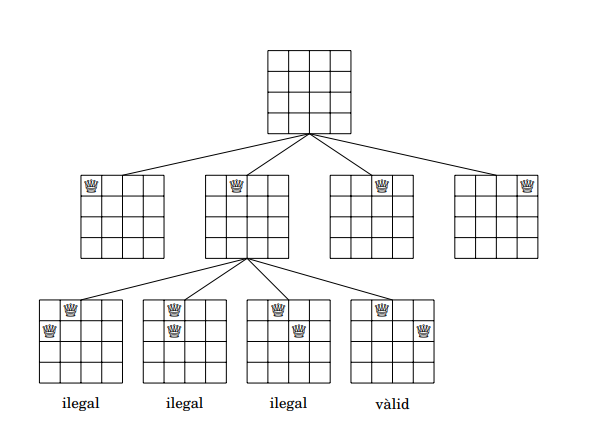
\includegraphics[width=.8 \textwidth]{back.png}
    
    \caption{\emph{Figura 5: Petita part de l'arbre de possibilitats que genera el backtracking amb $n = 4$. Font: \url{https://cses.fi/book/book.pdf}}}
\end{center}



Un altre exemple de l'ús del backtracking és quan es vol imprimir tots els subconjunts que es poden formar a partir d’un conjunt de paraules.

Plantegem el problema com un llistat de booleans i per cada paraula hem de decidir amb veritat o fals si agafem la paraula o no, per fer-ho més entenedor ens ho hem d'imaginar de nou com un arbre en el qual si vas per la branca de l'esquerra, vol dir que no agafes la paraula en canvi si vas cap a la dreta, sí que l'agafes, finalment quan arribem al final d'una branca, imprimim el subconjunt.


\begin{center}
    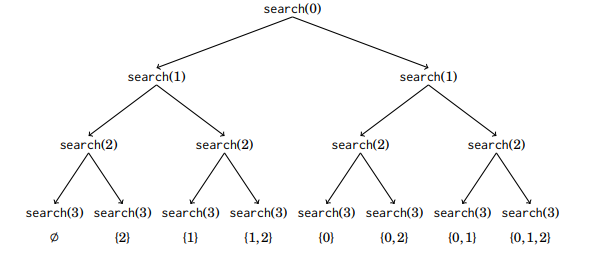
\includegraphics[width=.9 \textwidth]{back2.png}
    \caption{\emph{Figura 6: Arbre de decisions que es formaria amb un conjunt de números [0,1,2]. Font: \url{https://cses.fi/book/book.pdf}}}
\end{center}

\newpage

En el següent codi, observem la implementació de l'exemple mencionat anteriorment. \newline


\begin{lstlisting}
vector<string> paraules;

void backtracking(int i, vector<bool> bools){
    if (i == n) {   // cas base de la recursió
        cout << "{";
        for (int i = 0; i < n; i++)
            if (bools[i] == true)
                cout << paraules[i] << ", ";
        cout << "}" << endl;
        return;
    }
    bools[i] = 0;  // fem backtracking
    backtracking(i + 1, bools);  // cas recursiu
    bools[i] = 1;  // fem backtracking
    backtracking(i + 1, bools);  // cas recursiu
}

// Si el conjunt de paraules fos ["hola", "hi", "bonjour"]

// L'output seria el següent:
//  {}
//  {bonjour}
//  {hi}
//  {hi, bonjour}
//  {hola}
//  {hola, bonjour}
//  {hola, hi}
//  {hola, hi, bonjour}

// Observem que concorda amb la imatge anterior.
\end{lstlisting}







\subsection{Grafs}
%\subsection{Grafs}%
\subsubsection{Què són i vocabulari}

Un graf és un estructura de dades no lineal que consta de nodes/vèrtexs i arestes, les arestes són línies que connecten dos nodes qualsevols del graf (així i tot, a vegades una aresta pot connectar un node amb el mateix node). \newline

\begin{center}
    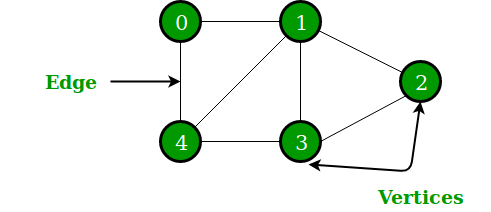
\includegraphics[width =.8 \textwidth]{graf.png}

    \caption{\emph{Figura 7: Exemple de graf. Font: \url{https://www.geeksforgeeks.org/difference-between-graph-and-tree/}}}
\end{center}

Per exemple, en el graf de la figura 7, els nodes són [0, 1, 2, 3, 4] i les arestes connecten els nodes [0-1, 0-4, 1-2, 1-3, 1-4, 2-3, 3-4]. \newline

Els grafs s'utilitzen recurrentment per resoldre problemes de la vida real i poden representar camins, carreteres, xarxes, etc.
Com a exemple de l'ús dels grafs a la vida quotidiana trobem les xarxes socials com Instagram, Facebook, etc. Cada usuari es representa com a un node que conté una estructura on es guarden les seves dades (id, nom, gènere, gustos, etc.) i a la vegada, aquest node està connectat amb altres nodes (seguidors, contactes, amics, etc.) mitjançant arestes. \newline

Un graf és connex si existeix un camí entre dos nodes qualssevol i no ho és si no es pot anar a un node qualsevol des d'un node inicial. \newline

\begin{center}
    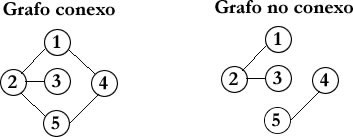
\includegraphics[width=.7 \textwidth]{GrafoConexo.jpg}

    \caption{\emph{Figura 8: Graf connex i graf no connex. Font: \url{https://www.unipamplona.edu.co/unipamplona/portalIG/home_23/recursos/general/11072012/grafo3.pdf}}}
\end{center}

\newpage

A la figura 8, apreciem que en el graf connex, podem anar a un node qualsevol des de qualsevol altre node, ja que tots els nodes estan connectats per arestes, en canvi, en el graf no connex contemplem que no podem anar a qualsevol node des de qualsevol altre node inicial. Per exemple, no es pot anar al node 5 des del node 1, puix que no hi ha un camí de nodes connexos units per arestes pels quals puguem assolir el node 5. \newline

A la figura 8, el graf connex consta d'una sola component connexa: [1,2,3,4,5].

A la figura 8, el graf no connex consta de dos components connexes: [1,2,3] i [4,5]. \newline \newline

Un graf conté un cicle si existeix algun recorregut o camí on el node inicial i el final sigui el mateix i sempre que ambdós nodes no siguin adjacents, és a dir, no estiguin connectats per una aresta. \newline

\begin{center}
    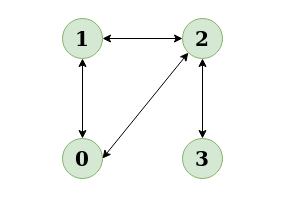
\includegraphics[width=.5 \textwidth]{GrafCicle.png}

    \caption{\emph{Figura 9: Graf amb cicle. Font: Propia}}
\end{center}

A la figura 9, observem que el graf conté un cicle, ja que podem fer el següent recorregut 0 -> 1 -> 2 -> 0 i, per tant, el node inicial i el final coincideixen (0), aquest fet causa que puguem entrar en un bucle infinit. \newline \newline

Un graf és un arbre si consta de $n$ nodes i $n-1$ arestes i no conté cap cicle, per tant, podem deduir que tan sols existeix un camí possible entre dos nodes qualsevols.

\begin{center}
    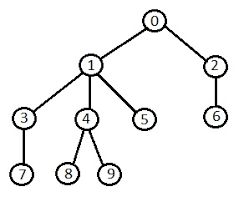
\includegraphics[width=.4 \textwidth]{TreeRoot.png}

    \caption{\emph{Figura 10: Graf (arbre). Font: \url{https://www.chegg.com/homework-help/questions-and-answers/consider-tree-tfe1png-answer-following-1-tis-rooted-vertex-2-siblings-vertex-3-3-parent-ve-q54883116}}}
\end{center}

Existeixen dues variacions de les arestes en els grafs: \newline

\textbf{Graf no dirigit:} les arestes del graf connecten dos nodes qualssevol per les dues bandes, és a dir, donats dos nodes $x$ i $y$, els quals estan connectats per una aresta, es pot anar tant des del node $x$ fins al $y$ com des del node $y$ fins al $x$, per tant, el graf es pot recórrer des de qualsevol node.

(Les arestes d'un graf no dirigit ens les podem imaginar com carreteres de doble sentit).
\newline

\textbf{Graf dirigit:} les arestes del graf només es poden recórrer en una direcció, és a dir, existeix una connexió entre els nodes x->y, però no entre y->x.

(Les arestes d'un graf no dirigit ens les podem imaginar com carreteres d'un únic sentit).

\begin{center}
    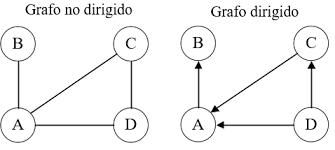
\includegraphics[width=.7 \textwidth]{GrafDir.png}
    
    \caption{\emph{Figura 11: Graf dirigit i graf no dirigit. Font: \url{https://www.researchgate.net/figure/Ejemplos-de-un-grafo-dirigido-y-un-grafo-no-dirigido_fig7_309278789}}}
\end{center}

Podem observar a la imatge que en el graf no dirigit, podem anar a qualsevol node des de qualsevol node, en canvi, en el graf dirigit, des del node B no poden anar enlloc jas que no disposa de cap connexió amb cap node. \newline

Per recórrer els grafs hi ha dos algorismes fonamentals: la cerca en profunditat, més coneguda com a DFS (depth-first search) o la cerca en amplada, més coneguda com a BFS (breadth-first search).

Els dos algorismes parteixen des d'un node inicial i després recorren tots els nodes als quals es poden arribar a partir d'aquest node inicial.

La diferència entre els dos algorismes és l'ordre amb el qual es recorren els nodes.

El que canvia entre la cerca en profunditat i la cerca en amplada i que en conseqüència provoca que l'ordre de visitar els nodes sigui diferent, és l'estructura de dades que utilitzen, la cerca en profunditat utilitza un stack (pila) o la recursió, en canvi, la cerca en amplada utilitza una queue (cua).


\subsubsection{Cerca en Profunditat (DFS)}

Com hem mencionat, aquest algorisme comença amb un node inicial, i continua per tots els altres nodes als quals es pot accedir des d'aquest node mitjançant les arestes del graf.

La cerca en profunditat sempre recorre un mateix camí, metres que hi hagi més nodes que no hàgem visitat i adjacents al node en el qual ens situem.

Quan això no es compleix, tornem als nodes anteriors i a partir d'aquests tornem a explorar fins que de nou no hi han més nodes no visitats adjacents al node en el qual ens situem, de nou tornem als nodes anteriors i així successivament fins que ja hem explorat tots els nodes que podíem explorar des del node inicial, cal recalcar que l'algorisme té control dels nodes que ja han estat visitats, de manera que processa un node tan sols una vegada, si no ho féssim així, podríem trobar-nos en un bucle infinit on anem d'un node A fins a un node B i a la inversa successivament fins a l'infinit.

Cal recalcar que la complexitat temporal de l'algorisme DFS és de $O(n+m)$ on $n$ representa el nombre de nodes i $m$ el nombre d'arestes en tot el graf.

\begin{center}
    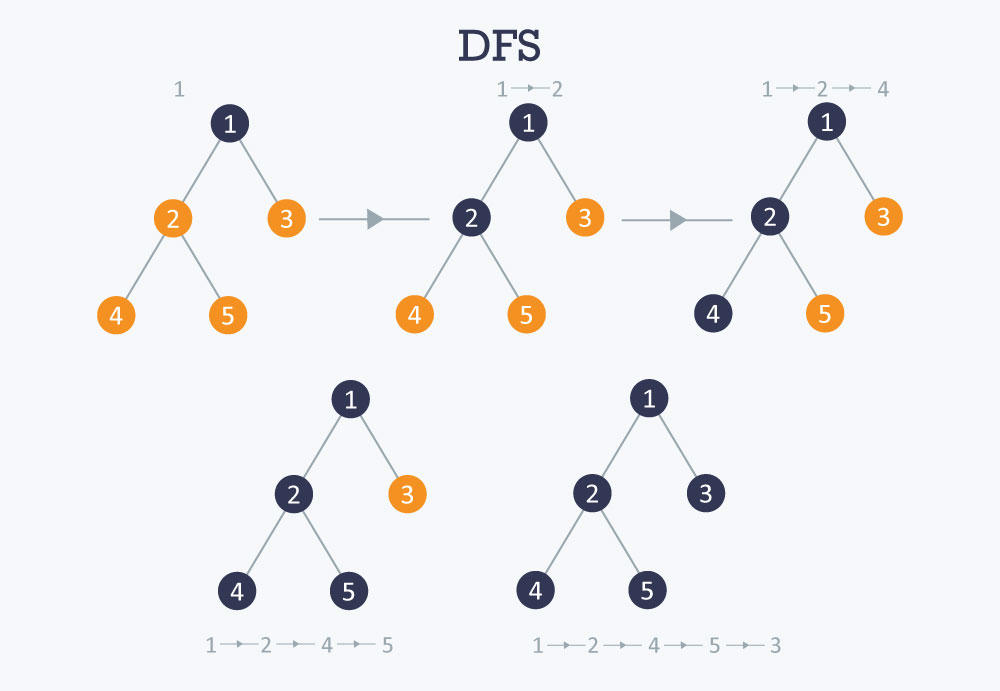
\includegraphics[width=.7 \textwidth]{GrafDFS.png}
    
    \caption{\emph{Figura 12: Exemple de DFS. Font: \url{https://www.hackerearth.com/practice/algorithms/graphs/depth-first-search/tutorial/}}}
\end{center}

A la figura 12, podem observar l'algorisme DFS en acció on els nodes negres representen nodes visitats i els taronges els no visitats, finalment tots acaben sent visitats. \newline

En els següents dos codis, considerem la implementació del DFS, primer utilitzant la recursió i seguidament utilitzant un $stack$ (pila).

\newpage

\begin{lstlisting}
// CODI DFS RECURSIÓ

vector<vector> adjacents; // Aquí guardem el graf
vector visitats; // Aquí guardem els nodes visitats

void DFS(int node){
    visitats[node] = true; // El marquem com a visitat
    for (auto nodeAdjacent : adjacents[node]) //Mirem nodes adjacents
        if (visitats[nodeAdjacent] == false) //Si no l'hem visitat
            DFS(nodeAdjacent); //Fem DFS amb el node adjacent
}

int main(){
    DFS(1); // Prenem el node 1 com a inicial
    
    for (int i = 0; i < n; i++)
        if (visitats[i] == true)
            cout << i << " "; // Imprimim tots els nodes visitats
}
\end{lstlisting}

\begin{lstlisting}
// CODI DFS PILA

vector<vector> adjacents; // Aquí guardem el graf
vector visitats; // Aquí guardem els nodes visitats

void DFS(){
    stack<int> pila;
    pila.push(1); // Prenem el node 1 com a inicial
    
    while (!pila.empty()){ // Mentres que puguem visitar nodes
        int node = pila.top(); // Agafem el node de dalt de la pila
        pila.pop(); // Traiem el node de la pila
        visitats[node] = true; // El marquem com a visitat
        for (auto nodeAdjacent : adjacents[node]) // Mirem nodes adjacents
            if (visitats[nodeAdjacent] == false) // Si no l'hem visitat
                pila.push(nodeAdjacent); // Afegim el node a la cua
    }
}

int main(){
    DFS();
    
    for (int i = 0; i < n; i++)
        if (visitats[i] == true)
            cout << i << " "; // Imprimim tots els nodes visitats
}

\end{lstlisting}
\newpage

En l'algorisme DFS primer es declaren els dos vectors essencials en els problemes de grafs: un vector d'adjacència (adjacents) on s'emmagatzema tots els nodes veïns o adjacents de cada node, un vector de nodes visitats (visitats) on es guarda el número de tots els nodes que ja s'han visitat per tal que un mateix node no sigui visitat infinitament i el programa acabi en un bucle sense fi.

Primerament, llegim el node inicial i l'afegim a la pila, per assegurar-nos que es visitin tots els nodes que es poden visitar a partir del node inicial, es declara en bucle que no pararà fins que la pila estigui completament buida, a cada pas del bucle s'agafa el node de sobre la pila, s'elimina d'aquesta i es marca com a visitat en el vector visitat, seguidament mitjançant un bucle s'agafen tots els veïns del node en el qual ens trobem i si no han estat visitats, els afegim a sobre la pila, finalment tots els nodes que podíem visitar ja han estat visitats i els imprimim.

L'algorisme DFS sempre forma un camí fins que arriba a un node en el qual tots els seus veïns ja han estat visitats gràcies a l'estructura de dades pila, ja que quan li afegim un altre node, aquest queda a sobre de tota la pila i, per tant, el següent pas del bucle serà des d'aquest node a causa del fet que sempre agafem el node que està a sobre de tota la pila.

Per entendre-ho millor, amb el següent graf (figura 13, faré una representació de com actuaria el DFS en aquest cas, en cada pas mostraré com seria la pila (la dreta representa el principi de la pila) i quins serien els nodes visitats.

\begin{center}
    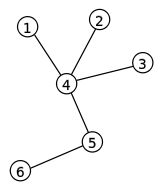
\includegraphics[width=.4 \textwidth]{tree.png}
    
    \caption{\emph{Figura 13: Graf (arbre). Font: \url{https://en.wikipedia.org/wiki/Tree_(graph_theory)}}}
\end{center}

Començarem per exemple pel node 1, l'afegim al començament de la pila. \newline

\textbf{Pila} [1]

\textbf{Visitat} [] \newline

Traiem el node 1 de la pila, l'afegim al vector visitat, mirem els seus nodes adjacents, afegim al començament de la pila el node 4. \newline

\textbf{Pila} [4]

\textbf{Visitat} [1] \newline

Traiem el node 4 de la pila, l'afegim al vector visitat, mirem els nodes adjacents al node 4, afegim els nodes 2, 3 i 5 al començament de la pila. \newline

\textbf{Pila} [2, 3, 5]

\textbf{Visitat} [1, 4] \newline

Traiem el node 5 de la pila, l'afegim al vector visitat, mirem els nodes adjacents al node 5, afegim al començament de la pila el node 6 i al vector visitats. \newline

\textbf{Pila} [2, 3, 6]

\textbf{Visitat} [1, 4, 5] \newline

Traiem el node 6 de la pila, l'afegim al vector visitat, mirem els nodes adjacents al node 6, no afegim cap node a la pila, ja que el seu node adjacent (5) ja ha estat visitat. \newline

\textbf{Pila} [2, 3]

\textbf{Visitat} [1, 4, 5, 6] \newline

Traiem el node 3 de la pila, l'afegim al vector visitat, mirem els nodes adjacents al node 3, no afegim cap node a la pila, ja que el seu node adjacent (4) ja ha estat visitat. \newline

\textbf{Pila} [2]

\textbf{Visitat} [1, 4, 5, 6, 3] \newline

Traiem el node 2 de la pila, l'afegim al vector visitat, mirem els nodes adjacents al node 2, no afegim cap node a la pila, ja que el seu node adjacent (4) ja ha estat visitat. \newline

\textbf{Pila} []

\textbf{Visitat} [1, 4, 5, 6, 3, 2] \newline

Com que la pila està buida, vol dir que ja hem visitat tots els nodes que podíem visitar i, per tant, el DFS finalitza.


\subsubsection{Cerca en Amplada (BFS)}

La cerca en amplada (breadth-first search) és molt semblant a la cerca en profunditat, però aquesta visita els nodes en ordre creixent a la seva distància des del node inicial. Així podem calcular molt fàcilment la distància des del node inicial fins a la resta de nodes, tanmateix, la cerca en amplada generalment és una mica més difícil d'implementar que la cerca en profunditat.

La cerca en amplada passa primer per tots els nodes els quals estan a una distància 1 del node inicial, és a dir que estan separats per una aresta, després pels que estan a una distància 2 i així successivament fins que tots els nodes ja han estat visitats.

\begin{center}
    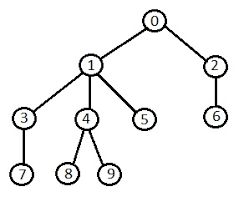
\includegraphics[width=.4 \textwidth]{TreeRoot.png}
    
    \caption{\emph{Figura 14: Graf (arbre). Font: \url{https://www.chegg.com/homework-help/questions-and-answers/consider-tree-tfe1png-answer-following-1-tis-rooted-vertex-2-siblings-vertex-3-3-parent-ve-q54883116}}}
\end{center}

Per exemple donat el graf de la figura 14, suposem que es pren com a node inicial el 0, llavors primerament visitem tots els nodes que estan a distància 1 del node 0, és a dir, visitem els nodes [1, 2], seguidament visitem els nodes [3, 4, 5, 6] i finalment visitem els nodes [7, 8, 9, 10].

Igual que la cerca en profunditat, la cerca en amplada té una complexitat temporal de $O(n + m)$, on $n$ és el nombre de nodes i $m$ el nombre d'arestes. \newline

En la següent implementació de l'algorisme BFS, recorrem tots els nodes que podem assolir des d'un node inicial a la vegada que ens guardem la distància a la qual estan tots els nodes del node inicial en un graf connex i no dirigit. \newpage


\begin{lstlisting}
vector<vector<int>> adjacents;  // Aquí guardem el graf
vector<bool> visitats;          // Aquí guardem els nodes visitats
vector<int> dist;               // Aquí guardem les distàncies

void BFS(){
    queue<int> cua;
    cua.push(1);   // Prenem el node 1 com a inicial    
    dist[1] = 0;   // Marquem distància 0 al node inicial
    
    while (!cua.empty()){ // Mentre que puguem visitar nodes
        int node = cua.front(); // Agafem el node del principi de la cua
        cua.pop();  // Traiem el node de la cua
        visitats[node] = 1; // Marquem el node com a visitat
        for (auto nodeAdjacent : adjacents[node]){ // Mirem nodes adjacents
            if (visitats[nodeAdjacent] == false){ // Si no l'hem visitat
                cua.push(nodeAdjacent);  // L'afegim a la cua
                dist[nodeAdjacent] = dist[node] + 1; 
                // La distància és igual a la del node del qual venim + 1
            }
        }
    }
}

int main(){ 
    BFS();  

    for (int i = 0; i < n; i++)
        if (visitats[i] == true)
            cout << dist[i] << " "; 
            // Imprimim les distàncies dels nodes visitats
}
\end{lstlisting}


L'algorisme BFS sempre visita els nodes per ordre de distància des del node inicial gràcies a l'estructura de dades cua, ja que com que els nodes s'afegeixen al final de la cua i s'agafen del principi de la cua, no es seguirà un camí definit sinó que la cerca es realitza en amplada.

Per entendre-ho millor, amb el següent graf, faré una representació de com actuaria el BFS en aquest cas, en cada pas mostraré com seria la cua (la dreta representa el principi de la cua) i com seria el vector distàncies. \newpage



\begin{center}
    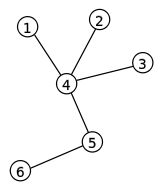
\includegraphics[width=.4 \textwidth]{tree.png}
    
    \caption{\emph{Figura 15: Graf (arbre). Font: \url{https://en.wikipedia.org/wiki/Tree_(graph_theory)}}}
\end{center}



Començarem per exemple pel node 1, l’afegim al final de la cua i li donem valor 0 a la distància. \newline

\textbf{Cua} [1]

\textbf{Dist} [1 : 0] \newline

Traiem el node 1 de la cua, mirem els nodes adjacents el node 1, afegim al final de la cua el node 4. \newline

\textbf{Cua} [4]

\textbf{Dist} [1 : 0] \newline

Traiem el node 4 de la cua, li donem valor 1 a la distància, mirem els seus nodes adjacents, afegim els nodes 2,3 i 5 al final de la cua. \newline

\textbf{Cua} [2, 3, 5]

\textbf{Dist} [1 : 0, 4 : 1] \newline

Traiem el node 5 de la cua, li donem valor 2 a la distància, mirem els seus nodes adjacents, afegim el node 6 al final de la cua. \newline

\textbf{Cua} [6, 2, 3]

\textbf{Dist} [1 : 0, 4 : 1, 5 : 2] \newline

Traiem el node 3 de la cua, li donem valor 2 a la distància, mirem els seus nodes adjacents, no afegim cap node a la cua, ja que el seu node adjacent (4) ja ha estat visitat. \newline

\textbf{Cua} [6, 2]

\textbf{Dist} [1 : 0, 3 : 2, 4 : 1, 5 : 2] \newline

Traiem el node 2 de la cua, li donem valor 2 a la distància, mirem els seus nodes adjacents, no afegim cap node a la cua puix que el seu node adjacent (4) ja ha estat visitat. \newline

\textbf{Cua} [6]

\textbf{Dist} [1 : 0, 2 : 2, 3 : 2, 4 : 1, 5 : 2] \newline

Traiem el node 6 de la cua, li donem valor 3 a la distància, mirem els seus nodes adjacents, no afegim cap node a la cua, ja que el seu node adjacent (5) ja ha estat visitat. \newline

\textbf{Cua} []

\textbf{Dist} [1 : 0, 2 : 2, 3 : 2, 4 : 1, 5 : 2, 6 : 3] \newline

Com que la cua està buida, vol dir que ja hem visitat tots els nodes que podíem visitar i, per tant, el BFS finalitza.



\subsubsection{Dijkstra}

L'algorisme Dijkstra's és un algorisme que ens serveix per trobar el camí més curt des del node inicial fins a tots els nodes del graf. \newline

Suposant que les arestes tenen llargades, quan ens referim al camí més curt no ens referim al camí on hem de travessar menys arestes sinó al camí el qual la llargada total de les arestes per les quals passem és la més curta. \newline

Per entendre-ho millor, imaginem que volem anar a París, Anglaterra i Roma des de Barcelona (les ciutats representen nodes i les carreteres arestes), per fer-ho hem de passar per moltes ciutats intermediàries i hi ha moltes maneres diferents d'arribar-hi, però nosaltres volem agafar el camí en el qual la distància total entre ciutats intermediàries sigui mínima per tal de recórrer el menor nombre de quilòmetres, esbrinar-ho seria una feina molt tediosa, ja que hi ha masses carreteres i combinacions possibles, per sort tenim el Google Maps que amb l'ús de l'algorisme Dijkstra's ja ho resol. \newline

Posarem com a exemple el funcionament de l'algorisme Dijkstra amb el següent graf (figura 16).

(En vermell les distàncies fins a cada node, en negre el nombre del node i distància de cada aresta)
\newline

\begin{center}
    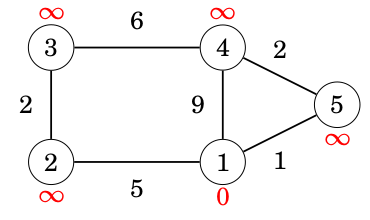
\includegraphics[width=.5 \textwidth]{grafDij1.png}
    
    \caption{\emph{Figura 16: Graf amb llargades. Font: \url{https://cses.fi/book/book.pdf}}}
\end{center}

Primerament, guardem distància infinita a tots els nodes menys al node inicial, que li posem distància 0.

A cada pas, l'algorisme escull un node que no ha estat processat encara i que la seva distància és la menor possible. En aquest cas seleccionem el node 1.

Cada vegada que un node és seleccionat, l'algorisme travessa totes les arestes que comencen al node i escurça les distàncies cap a altres nodes mitjançant aquestes:

\begin{center}
    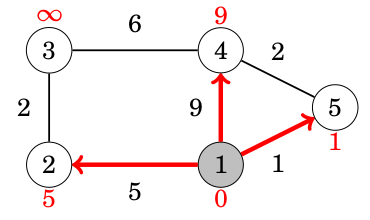
\includegraphics[width=.5 \textwidth]{grafDij2.png}
    
    \caption{\emph{Figura 17: Graf amb llargades. Font: \url{https://cses.fi/book/book.pdf}}}
\end{center}

En aquest cas, les arestes del node 1 han reduït les distàncies fins als nodes 2,4 i 5 que ara passen a ser 5,9 i 1.

Seguidament, processem el node 5, que ens redueix la distància fins al node 4 de 9 fins a 3, ja que és més òptim fer un camí de distància 2+1 = 3 que de distància 9.

\begin{center}
    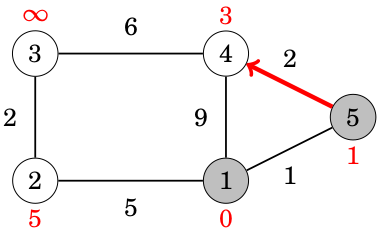
\includegraphics[width=.5 \textwidth]{grafDij3.png}
    
    \caption{\emph{Figura 18: Graf amb llargades. Font: \url{https://cses.fi/book/book.pdf}}}
\end{center}

Ara toca processar el node 4 que ens redueix la distància fins al node 3.

\begin{center}
    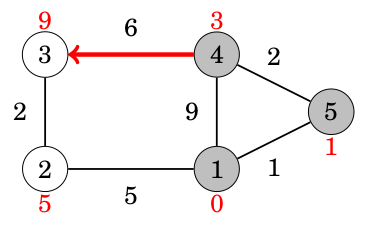
\includegraphics[width=.5 \textwidth]{grafDij4.png}
    
    \caption{\emph{Figura 19: Graf amb llargades. Font: \url{https://cses.fi/book/book.pdf}}}
\end{center}

Aquest procés el repetim dues vegades més amb els nodes 2 i 3, finalment obtindríem les distàncies òptimes cap a tots els nodes i el graf quedaria de la següent manera.

\begin{center}
    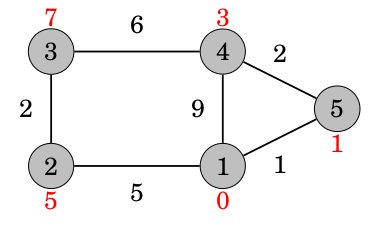
\includegraphics[width=.5 \textwidth]{grafDij5.png}
    
    \caption{\emph{Figura 20: Graf amb llargades. Font: \url{https://cses.fi/book/book.pdf}}}
\end{center}

La següent implementació de l'algorisme de Dijkstra calcula les distàncies mínimes des d'un node $x$ als altres nodes del graf.

Una implementació eficient de l'algorisme de Dijkstra requereix trobar de manera eficient el node de distància mínima que no s'ha processat encara. L'estructura de dades adequada és una cua de prioritats que conté els nodes ordenats per distància. Amb una cua de prioritats trobem el següent node a processar en temps $O(\log n)$.

El graf s'emmagatzema com a llistes d'adjacència de manera que $adj[a]$ conte un parell $(b, w)$ quan hi ha una aresta del node $a$ fins al node $b$ amb pes $w$.

El vector $dist$ conte la distància a cada node.

Inicialment, la distància és 0 al node inicial i $\infty$ a tots els altres nodes.

\begin{lstlisting}
vector<vector<pair<int,int>>> adj; // llista d'adjacència
vector dist; // llista de distàncies
int INF = 10e9;

for (int i=1; i<n; i++)
    dist[i] = INF; // marquem distància infinita a
                   // tots els nodes menys el 0

priority_queue<pair<int,int>> cua; // distància - node
cua.push({0, 0}); // afegim a la cua node 0 amb distància 0

// comencem el Dijkstra's

while (!cua.empty()){
    int nodeActual = cua.top().second; 
    // agafem el node amb menys distància
    int distanciaActual = cua.top().first
    cua.pop(); // traiem el node de la cua
    
    if (abs(distanciaActual) > dist[nodeActual]) continue;
    // si el valor absolut de la distància del nodeActual és menor,
    // no la volem actualitzar
    
    for (auto u : adj[nodeActual]){ // mirem els nodes adjacents
        int nodeAdjacent = u.first;
        int distancia = u.second;
        
        if (dist[nodeActual] + distancia < dist[nodeAdjacent]){
            // si podem acurtar la distancia al nodeAdjacent mitjançant
            // el nodeActual, l'actualitzem
            dist[nodeAdjacent] = dist[nodeActual] + distància;
            // afegim la nova distància i el nodeAdjacent
            cua.push({-dist[nodeAdjacent], nodeAdjacent});
        }
    }
}

\end{lstlisting}

Cal recalcar que la complexitat temporal de la implementació anterior és $O(n + m \log m)$, per
què l'algorisme passa per tots els nodes del graf i afegeix, per cada aresta, com a màxim una distància a la cua de prioritats.


\part{Marc Pràctic}
\section{Força Bruta A La Vida Real}

Durant el dia, emprem concurrentment l'algorisme de força bruta, ja que aquest, encara que pugui trigar molt a donar-nos una solució, sempre en troba una.

Per exemple, quan som petits i els nostres pares ens deixen el clauer per obrir la porta de casa, nosaltres no sabem quina és la clau bona, per tant, emprem la força bruta, bàsicament provem d'obrir la porta a cada clau fins que alguna ens obre la porta, utilitzem aquest mètode, ja que sabem que sempre trobarem la clau bona.

A la vida real, en l'àmbit de la tecnologia, la força bruta s'utilitza recurrentment en el pirateig.

Cal recalar que quasi tots els problemes que podem trobar es poden resoldre amb la força bruta, per exemple un problema de grafs en el qual hàgem de trobar el camí més curt des d'un node $x$ a un node $y$, també es pot resoldre amb força bruta, puix que podem provar tots els camins possibles i agafar el més curt, tot i això, aquest algorisme tindria una complexitat temporal de $O({n\displaystyle !\,})$ i per tant si $n = 50$, un valor realment petit, la força bruta faria aproximadament unes $3 \cdot 10^{64}$ operacions, un nombre totalment desorbitat.

Com a exemple pràctic, imitaré un algorisme de força bruta que utilitzen els pirates informàtics per endevinar una contrasenya (que pot contenir tota classe de caràcters) de secreta d'un usuari.

\begin{lstlisting}
int main(){
    string caractersPossibles "!#$%&\'()*+,-./0123456789:;<=>?@ABCDE
    FGHIJKLMNOPQRSTUVWXYZ[\\]^_'abcdefghijklmnopqrstuvwxyz{|}~";
    
    int maximaLlargada = 16;
    
    string contrasenyaUsuari = "abc123#";
    
    do {
        // miro totes les possibles permutacions
        // de tots els caràcters
        string contrasenyaProva = "";
        for (int i = 1; i <= maximaLlargada; i++){
            // provo una contrasenya per cada
            // llargada possible
            contrasenyaProva += caractersPossibles[i];
            
            if (contrasenyaProva == contrasenyaUsuari) {
                // les contrasenyes coincideixen
                cout << "He trobat la teva contrasenya !"
                return 0;
            }
        
        }
    } while (next_permutation(caractersPossibles.begin(), 
      caractersPossibles.end());

}
\end{lstlisting}

Cal recalcar que la complexitat d'aquest algorisme és de $O(maximaLlargada * 93!)$, uns números vertiginosos, és per això que els pirates informàtics optimitzen relativament els seus algorismes de força bruta.
\subsection{Problemes Força Bruta}

\textbf{Problema 1:} \newline

Dificultat -> fàcil. \newline

\textbf{Enunciat:} \newline

Estem jugant un videojoc i hem de derrotar $n$ monstres, els quals estan formant una rotllana i numerats de l'1 fins a $n$.

Al començament, el $i-esim$ monstre té $vida_{i}$ vida.

Per derrotar els monstres tenim bales, cada bala redueix la vida del monstre que hem disparat en 1. A més a més, quan la vida d'algun monstre $i$ esdevé 0, aquest explota, realitzant així $mal_{i}$ de mal al monstre de la dreta (és a dir al monstre $i + 1$ si $i < n$ o al monstre $1$ si $i == n$, o millor dit, al ($(i + 1) \mod n$) monstre), si l'explosió mata al monstre de la dreta, llavors aquest també explota i així successivament. \newline

La tasca consisteix a trobar el mínim nombre de bales que hem de disparar per tal que tots els monstres siguin derrotats.

Ens asseguren també que $(2\leq n \leq 3 \cdot 10^5)$.

Aquesta informació és molt important, ja que ens informa del fet que la nostra solució pot tenir com a màxim una complexitat de $O(n \cdot \log n)$. \newline

\textbf{Idea:} \newline

La idea principal per resoldre aquest problema és que no podem aprofitar el mal de l'explosió de l'últim monstre que matem, per tant, hem de trobar el monstre que matant-lo l'últim, hem de disparar el mínim nombre de bales, llavors primerament hem de calcular la vida que li queda a cada monstre després què l'anterior monstre exploti, per trobar aquest valor hem de fer la següent operació: $max(0, vida_{i} - mal_{i-1})$, aquest valor serà les bales que haurem de disparar per matar al $i-esim$ monstre, menys pel primer, que haurem de disparar $a_{i}$ bales, ja que tindrà tota la vida.

\newline

Per tant, per trobar la millor solució, ho haurem de fer mitjançant la força bruta i haurem de trobar l'índex $i$ tal que $a_{i}$ - $max(0, a_{i} - b_{i - 1})$ és el mínim possible.

\textbf{Implementació:}

\begin{lstlisting}
int n; cin >> n;
// número de monstres

vector vida(n);
// vida de cada monstre inicialment
vector mal(n);
// mal que fa cada monstre a l'explotar
vector vida_restant(n);
// vida restant de cada monstre quan explota l'anterior monstre

for (int i = 0; i < n; i++)
    cin >> vida[i] >> mal[i];
// llegeixo el vector

int suma = 0;
// suma de la vida restant total

for (int i = 0; i < n; i++){
    vida_restant[(i + 1) % n] = max(0ll, vida[(i + 1) % n] - mal[i]);
    // calculem la vida restant de cada monstre quan explota
    // l'anterior monstre
    suma += vida_restant[(i + 1) % n];
    // afegim la vida restant a la suma
}

int minim = (1ll << 62); // (2 ^ 62)
// donem valor molt gran al mínim perquè els valors
// calculats siguin menors

for (int i = 0; i < n; i++){
    minim = min(minim, vida[i] - vida_restant[i]);
    // agafem el valor més petit
}

cout << minim + suma << endl;
// el resultat és el valor mínim més la suma
\end{lstlisting}


\section{Algorismes Greedy A La Vida Real}

La majoria de decisions que prenem en el nostre dia i en la vida en general, segueixen una estratègia $Greedy$, ja que quasi sempre intentem prendre la decisió que més ens beneficia en el moment de prendre aquesta. \newline

Per exemple, a l'hora de completar un examen, una estratègia $Greedy$ podria consistir a resoldre els exercicis en ordre creixent de dificultat (primer els més fàcils i finalment els més difícils).

Un altre exemple, quan anem a comprar qualsevol classe de producte, una estratègia $Greedy$ podria consistir a comprar la marca més econòmica d'aquell producte, ja que així estalviem diners, una altra estratègia $Greedy$ possible seria comprar la marca més cara del producte, puix que així, probablement estem agafant un producte de major qualitat. \newline

En poques paraules, a l'hora de prendre una decisió, tenim innumerables estratègies $Greedy$ possibles a seguir i quasi mai cap és cent per cent correcte.
\newline



Un exemple quotidià de l'ús de l'algorisme $Greedy$, és quan anem a comprar i volem pagar amb el menor nombre de monedes possibles.

Si per exemple hem de pagar 163 cèntims, primer busquem la moneda més gran que tinguem que no sobrepassi els 163 cèntims, si tinguéssim tots els valors de monedes, primer pagaríem 1 euro (100 cèntims), ens restarien 63 cèntims a pagar i de nou busquem la moneda més eficient, en aquest cas seria una moneda de 50 cèntims, ens quedarien 13 cèntims a pagar, altra vegada busquem la moneda més gran que no sobrepassi la xifra de 13 cèntims que seria la moneda de 10 cèntims, ens quedaran tan sols 3 cèntims a pagar que no ens quedaria més remei que pagar-los amb 1 moneda de 2 cèntims i 1 moneda d'1 cèntim.
\newline

En aquest cas l'estratègia $Greedy$ consisteix a agafar la moneda més gran que no sobrepassi els diners restants a pagar. Amb el sistema de monedes a España, aquesta estratègia és l'òptima sempre, però si tinguéssim monedes de tots els cèntims possibles, aquesta estratègia no funcionaria sempre, per exemple:

Si tenim les següents monedes [1,3,4] (cèntims) i hem de pagar 6 cèntims, doncs amb l'estratègia $Greedy$ anterior, agafaríem les següents monedes [4,1,1] però realment l'opció més bona seria agafar les següents monedes [3,3].

Per resoldre aquest problema de manera òptima amb monedes de qualsevol valor, haurem d'utilitzar la \emph{programació dinàmica} (la veurem més endavant). \newpage

En el següent codi, podem observar la implementació de l'estratègia $Greedy$ de la qual hem parlat.
\newline

\begin{lstlisting}
int main(){
    int preu_total;
    cin >> preu_total; // Input -> 279
    int preu_a_pagar = preu_total;
    
    vector<int> monedes = {200,100,50,20,10,5,2,1};
    vector<int> monedes_utilitzades;
    int index = 0;
    int monedes_pagades = 0;
    
    while (preu_a_pagar > 0){
        if (preu_a_pagar >= monedes[index]){
            preu_a_pagar -= monedes[index];
            monedes_utilitzades.push_back(monedes[index]);
            monedes_pagades++;
        } else {
            index++;
        }
    }
    cout << "Hem pagat: " << preu_total << " cèntims amb: "
    << monedes_pagades << " monedes." << endl;
    cout << "{";
    for (auto e : monedes_utilitzades){
        cout << e << ",";
    cout << "}";
    
    // Output -> Introdueix el preu a pagar: Hem pagat: 279 cèntims amb:
    // 6 monedes {200,50,20,5,2,2}
}

\end{lstlisting}
\subsection{Problemes Greedy}

\textbf{Problema 1:} \newline

Dificultat -> mitjana. \newline

\textbf{Enunciat:} \newline

Tenim un carrer amb $n$ cases, on la $i-esima$ casa està pintada de color $actual_{i}$; així i tot, volem que la $i-esima$ casa estigui pintada de color $esperat_{i}$, per intentar complir el nostre desig, hem convidat a $m$ pintors, el $j-esim$ pintor arriba al moment $j$ i ha de repintar exactament una casa del color $color_{j}$.

Podem repintar totes les cases amb els colors esperats?, si és que si, hem d'imprimir $m$ números, on el $j-esim$ número és la $m_{j}$-$esima$ casa pintada pel $j-esim$ pintor i del color $color_{j}$. \newline

Ens asseguren també que $(1\leq n \leq 10^5)$.

Aquesta informació és molt important, ja que ens informa que la nostra solució pot tenir com a màxim una complexitat d'aproximadament $O(n \cdot \log n)$. \newline

\textbf{Idea:} \newline

Per resoldre el problema, primer ens hem d'adonar que l'últim pintor és el més rellevant (i pintarà la $x-esima$ casa, on $esperat_{x} = colors_{m}$), ja que així podem pintar la $x-esima$ casa dels colors que no vulguem i finalment amb l'últim color, la pintarem del color que volem.

Llavors primer intentem trobar una casa on $esperat_{x} = colors_{m}$ i $actual_{x}$ != $esperat_{x}$, ja que així estem aprofitant una casa que ja havíem de pintar de totes formes, si no trobem una casa que compleixi aquestes dues condicions, intentem trobar una casa on $esperat_{x} = colors_{m}$, si no trobem una casa que compleixi aquesta condició vol dir que no existeix cap solució.

Seguidament, hem de repartir de forma $Greedy$ els $m$ colors, i ho fem de la següent manera:

\begin{itemize}
\item Si hi ha una casa $i$, tal que $esperat_{i}$ = $color_{j}$ i $actual_{i}$ != $esperat_{i}$, llavors pintarem la $i-esima$ casa del $j-esim$ color.
\item Si hi ha una casa $i$, tal que $esperat_{i}$ = $color_{j}$ i $actual_{i}$ != $esperat_{i}$, llavors pintarem la $x-esima$ casa del $j-esim$ color.
\end{itemize}

Finalment, tan sols ens queda comprovar si la quantitat de cada color dels colors que tenim és major a la quantitat de cada color dels colors que necessitem.

Si aquesta última condició no es compleix, llavors vol dir que no existeix cap solució total. \newline

\textbf{Implementació:} \newline

\begin{lstlisting}
int n,m; cin >> n >> m;
// n = número de cases
// m = número de pintors

vector actual(n);
// color de les cases al principi
vector esperat(n);
// color de les cases que volem
vector colors(m);
// color de les pintures
vector solucio(m);
// aqui guardem la solucio
map<int,int> tinc;
// els colors que tinc al principi
map<int,int> necessito;
// els colors que necessito al final
map<int,bool> util;
// els colors que són útils
vector<vector> posicions(n+1);
// les posicions de les cases de cada color que cal canviar

for (int i=0; i<n; i++)
    cin >> actual[i];
// llegeixo el vector

for (int i=0; i<n; i++){
    cin >> esperat[i];
    // llegeixo el vector
    util[esperat[i]] = true;
    // marco com a útil el valor esperat[i]
    // ja que és un color que necessito
    
    if (actual[i] != esperat[i]) {
        // si el color al principi és diferent del color final
        posicions[esperat[i]].push_back(i);
        // l'afegeixo al vector
        necessito[esperat[i]]++;
        // sumo 1 al color que necessito canviar
    }
}

for (int i=0; i<m; i++){
    cin >> colors[i];
    // llegeixo el vector
    tinc[colors[i]]++;
    // sumo 1 al color que puc canviar
}

bool pot = util[colors[m-1]];
// bool per saber si existeix una solució de primeres
// mirem si l'últim color és útil o no
bool f = 1;
// bool per saber si existeix una solució total
int col = colors[m-1];
// últim color dels colors
int it = -1;
// iterador per saber quina casa és la que volem canviar
// si el color no és útil

if (!pot) {
    // si pot és fals, no hi ha cap solució total
    f = 0;
} else {
    // construïm la solució
    for (int i=0; i<n; i++){
        if (actual[i] != esperat[i] && esperat[i] == col){
            // si hem de canviar de color la casa
            // i el color esperat és el mateix que col
            it = i;
            // donem valor i a l'iterador it
            break;
            // aturem el bucle
        }
    }
    if (it == -1){
        // si no hem satisfet la condició del bucle anterior
        for (int i=0; i<n; i++){
            if (esperat[i] == col)
                // si coincideixen el color
                it = i;
                // donem valor i a l'iterador it
        }
    }
    
    for (int i=0; i<m; i++){
        if (!posicions[colors[i]].size()){
            // si el color no és útil o bé no queden
            // mes cases per pintar d'aquell color
            solucio[i] = it + 1;
            // pintem la casa it
        } else {
            // si queden cases per pintar d'aquest color
            int pos = posicions[colors[i]].back();
            posicions[colors[i]].pop_back();
            solucio[i] = pos + 1;
            // pintem la casa pos d'aquest color
        }
    }
}

// comprovo si la solució és correcta
for (auto x : necessito)
    if (tinc[x.first] < necessito[x.first])
        // si necessito més colors dels que tinc
        // llavors la solució és incorrecta
        f = 0;

if (f) {
    // si hem trobat una solució total
    cout << "YES" << endl;
    for (int i=0; i<m; i++)
    cout << solucio[i] << " ";
    // imprimim la solució
    cout << endl;
} else {
    // si no hem trobat una solució
    cout << "NO" << endl;
    // simplement imprimim NO
}

\end{lstlisting}


\section{Cerca Binària A La Vida Real}

La cerca binària, a diferència del que puguem pensar, és un dels algorismes més presents en les nostres vides, per exemple, imaginem que estem comprovant la resistència d'un telèfon mòbil a les altures, primerament podríem pensar que per fer-ho podem primer tirar un mòbil des del primer pis d'un bloc de pisos i anar pujant pisos fins que arribem a un pis des del qual quan tirem el mòbil, aquest es trenca, llavors sabem que la màxima altura des del que podem tirar el telèfon mòbil és l'altura a la qual està l'anterior pis.

Tot i així, a la vida real, en comptes d'anar provant cada pis, aplicaríem la cerca binària per tal de tirar els menys telèfons mòbils possibles. \newline

\begin{lstlisting}
int Pis_Minim = 0, Pis_Màxim = 100;

while (Pis_Màxim > Pis_Minim + 1){
    int Pis_Entremig = (Pis_Minim + Pis_Màxim) / 2;

    bool Trenca_Mòbil; // comprovem si es trenca el mòbil des d'aquell pis
    if (Trenca_Mòbil == true){
        // si el mòbil es trenca des del pis entremig, llavors podem
        // assegurar que des de tots els pisos per sobre d'aquest
        // el mòbil també es trencarà
        Pis_Màxim = Pis_Entremig;
    } else {
        // si el mòbil no es trenca des del pis entremig, llavors podem
        // assegurar que des de tots els pisos per sota d'aquest
        // el mòbil no es trencarà
        Pis_Minim = Pis_Entremig;
    }
}

// Finalment, el pis màxim des del qual el mòbil no es trenca
// és el Pis_Minim

cout << Pis_Minim << endl;
\end{lstlisting}

La cerca binària vista en l'anterior codi, és la que aplicaríem a la vida real, d'aquesta manera minimitzaríem els intents i, per tant, els telèfons mòbils que hem de tirar. \newline

Posem un altre exemple, imaginem que som una empresa de vidres blindats i volem trobar quina és la distància màxima a la qual el nostre vidre blindat resisteix una bala amb el mínim nombre de dispars possibles.

Sabem que una bala disparada a una distància de 0 metres trenca el vidre i que una bala a 101 metres no.

Per tal de disparar el menor nombre de vegades, primer disparem a una distància de 50 metres, puix que
$ \lfloor (1 + 100) / 2 \rfloor $ = $ \lfloor 50.5 \rfloor $ = 50, imaginem que el vidre es trenca, llavors reduïm l'interval a 51-100, ja que si el vidre es trenca a una distància de 50 metres, sabem que a les distàncies entre 1 i 49 metres, el vidre també es trencarà i, per tant, seria inútil comprovar aquelles distàncies.

Seguidament, dispararíem una bala a una distància de 75 metres, ja que $ \lfloor (51 + 100) / 2 \rfloor $ = $ \lfloor 75.5 \rfloor $ = 75, ara imaginem que el vidre no es trenca, en aquest cas reduïm l'interval a 51-74, ja que si el vidre no es trenca a una distància de 75 metres, no cal dir que a les distàncies entre 76 i 100 metres, el vidre tampoc es trencarà i, per tant, seria inútil comprovar aquelles distàncies.

Aquest procés el repetiríem fins que arribem a un interval $X - Y$ en el qual X = Y - 1 i, per tant, la distància màxima a la qual el vidre blindat resisteix una bala és $Y$.


\subsection{Problemes Cerca Binària}

\textbf{Problema 1:} \newline

Dificultat -> mitjana. \newline

\textbf{Enunciat:} \newline

Ens donen les coordenades $X$ de $n$ ciutats i de $m$ centrals de wifi, les quals aporten senyal a les ciutats que estan a una distància de com a màxim $r$.

La tasca és trobar la $r$ mínima de les centrals per tal que cada ciutat tingui almenys una central que li proporcioni senyal.

Ens asseguren també que $(1\leq n, m \leq 10^5)$ i que les coordenades de les ciutats i de les centrals
$(1\leq ciutat_{i}, central_{i} \leq 10^9) $.

Aquesta informació és molt important, puix que ens informa que la nostra solució pot tenir com a màxim una complexitat de $O(n \cdot \log n)$, també ens informa que la $r$ màxima és de $10^9$. \newline

\textbf{Idea:} \newline

Per resoldre el problema, farem una cerca binària de $r$ i llavors comprovarem si amb el punt mitjà $m$ de la cerca binària podem donar senyal a totes les ciutats, si és que si, llavors augmentarem l'interval esquerre fins a $m$, per contra, si és que no, llavors reduirem l'interval dret a $m$, finalment la resposta serà l'interval dret.
\newline

\textbf{Implementació:} \newline

\begin{lstlisting}
int n, m; // nombre de ciutats i centrals
 
vector<int> ciutats;  // vector amb coordenades X de ciutats
vector<int> centrals;  // vector amb coordenades X de centrals
 
bool check(int r){
    int ciutat_Actual = 0;  // iterador ciutat actual
    int central_Actual = 0;  // iterador central actual
    
    // mentrestant que no haguem usat totes les centrals o ciutats
    while (ciutat_Actual < n && central_Actual < m){
    
        if (centrals[central_Actual] + r >= ciutats[ciutat_Actual] && 
        centrals[central_Actual] <= ciutats[ciutat_Actual]) {
        
            // si la central actual pot proporcionar senyal a la
            // ciutat actual llavors passem a la següent ciutat
            ciutat_Actual++;
        } else if(centrals[central_Actual] - r <= ciutats[ciutat_Actual] &&
        centrals[central_Actual] >= ciutats[ciutat_Actual]){
        
            // si la central actual pot proporcionar senyal a la
            // ciutat actual llavors passem a la següent ciutat
            ciutat_Actual++;
        } else {
        
            // si la central actual NO pot proporcionar senyal a la
            // ciutat actual llavors passem a la següent ciutat
            central_Actual++;
        }
    }
    // Si hem cobert les n ciutats amb senyal, retornem true, sinó, false
    return ciutat_Actual == n;
    
}

signed main(){
    cin >> n >> m; // llegim n i m
    
    ciutats.resize(n); // actualitzem la capacitat del vector ciutats
    centrals.resize(m); // actualitzem la capacitat del vector centrals
    
    for (int i = 0; i < n; i++){
        cin >> ciutats[i]; // llegim les coordenades de les ciutats
    }
    
    for (int i = 0; i < m; i++){
        cin >> centrals[i]; // llegim les coordenades de les centrals
    }
    
    int dreta = 10e9;  // interval màxim de r
    int esquerra = -1; // interval mínim de r
    
    while (dreta > esquerra + 1){ // comença la cerca binària
        int mig = (dreta + esquerra) / 2; // agafem punt mig
        
        if (check(mig)){
            // si amb aquesta r podem donar senyal, minimitzem la dreta
            dreta = mig;
        } else {
            // si amb aquesta r NO podem donar senyal, augmentem l'esquerra
            esquerra = mig;
        }
    }
    cout << dreta << endl;
}
\end{lstlisting}

\newpage





\section{Programació Dinàmica A La Vida Real}

La programació dinàmica s'utilitza recurrentment en l'àmbit de la tecnologia: per exemple en xarxes informàtiques, encaminaments, problemes de grafs, visió artificial, inte\lgem igència artificial, aprenentatge automàtic, etc.

Així i tot, també trobem la programació dinàmica en els comerços i empreses, per exemple, l'encaminament d'enviaments als llocs web de comerç electrònic està modelat com un algorisme del camí més curt que empra la programació dinàmica.

Un altre exemple el trobem en l'optimització de l'embalatge de caixes en els grans magatzems, alguna vegada t'has preguntat com Amazon fa ús dels algorismes per decidir quin producte ha d'anar a quina capsa de cartó? La decisió de fer servir recursos eficients es resol amb la programació dinàmica.

Finalment, un exemple molt comú el trobem en la següent situació: demà tens un examen, no has estudiat res, però coneixes la probabilitat que entri una pregunta sobre cada tema que pot entrar a l'examen i també saps el temps aproximat que trigues a estudiar cada tema, per maximitzar la nota has d'escollir els temes les dubtes dels quals tenen una alta probabilitat d'aparèixer a l'examen; tot i això, també hem de tenir en compte els minuts necessaris per completar aquests temes i de no superar el temps total del qual disposes per estudiar.

El problema anterior és el conegut $problema de motxilla$ i es resol amb la programació dinàmica.

A continuació, observem el codi per maximitzar la probabilitat total del fet que entri cada tema per treure la màxima nota possible. \newline

\begin{lstlisting}
int temps_estudi = 120;
// temps total per estudiar
int numero_temes = 5;
// numero total de temes que entren a l'examen

vector<pair<int,int>> temes = {{0, 0}, {40, 80},
{90, 100}, {50, 60}, {30, 20}, {80, 90}};
// temps per estudiar cada tema - percentatge que entri
// el tema a l'examen

vector<vector> dp(numero_temes + 1, vector(temps_estudi + 1, 0));
// dp[i][j] = màxim percentatge que es pot aconseguir
// estudiant com a màxim els primers i temes
// estudiant com a màxim durant j minuts

for (int i = 1; i <= numero_temes; i++){
    for (int j = 1; j <= temps_estudi; j++){
        dp[i][j] = max(dp[i][j], dp[i - 1][j]);
        // com a mínim, dp[i][j] = dp[i - 1][j]
        // ja que podem aconseguir el mateix percentatge
        if (j >= temes[i].first)
            // si ha passat suficient temps perquè puguem estudiar
            // el i-esim tema
            dp[i][j] = max(dp[i][j], dp[i - 1][j - temes[i].first]
        + temes[i].second);
            // mirem si estudiant el i-esim tema, estem maximitzant
            // el percentatge
    }
}
cout << dp[numero_temes][temps_estudi] << endl;
\end{lstlisting}


\subsection{Problemes Programació Dinàmica}

\textbf{Problema 1:} \newline

Dificultat -> mitjana. \newline

\textbf{Enunciat:} \newline

Ens donen un text $t$ i un conjunt de $n$ strings $strings_{1},strings_{2}....strings_{n}$.

L'objectiu és pintar $t$ de color vermell, per fer-ho, en un pas podem triar qualsevol ocurrència de qualsevol string $strings_{i}$ dins de $t$ i pintar la substring corresponent de $t$.

Per exemple si $t = casa$, $strings_{1} = sa$ i $strings_{2} = ca$, llavors podem pintar $t$ en dos passos, primer pintem la substring $ca$ de $t$ amb $strings_{2}$, $t$ quedaria de la següent manera: \textcolor{red}{ca}sa, finalment pintaríem la substring $sa$ de $t$ amb $strings_{1}$, $t$ quedaria de la següent manera: \textcolor{red}{casa}.

Si és impossible pintar totes les lletres de $t$, hem d'imprimir -1.

D'altra manera, hem d'imprimir $m$ (el mínim nombre de vegades que hem de pintar $t$).

Seguidament, hem d'imprimir $m$ línies, la $i-esima$ línia ha de contenir dos enters, $utilitzat_{j}$ (hem utilitzat la $j-esima$ string en el $i-esim$ pas) i $posició_{j}$ (hem començat a pintar des de la $j-esima$ en el $i-esim$ pas).
\newline

Ens asseguren que $(1\leq llargada_t \leq 100)$, $(1\leq n \leq 10)$, $(1\leq llargada_strings_{i} \leq 10)$.

Aquesta informació és molt important, ja que ens informa que la nostra solució pot tenir com a màxim una complexitat $O(llargada_t^2 \cdot n \cdot llargada_strings_{i})$. \newline

\textbf{Idea:} \newline

Per resoldre aquest problema farem servir la programació dinàmica, per fer-ho mantindrem un vector $dp$ en el qual $dp_{i}$ contindrà el mínim nombre de vegades que hem de pintar $t$, si pintem $t$ fins a la $i-esima$ lletra, també mantindrem un vector $previ$ en el qual $previ_{i}$ contindrà dos enters, $j_{i}$ (hem utilitzat $strings_{j}$ per pintar $t$ fins a la $i-esima$ lletra) i $llargada_{i}$ (hem utilitzat $llargada_{i}$ lletres de $strings_{j}$ per pintar $t$ fins a la $i-esima$ lletra). \newline

Cal recalcar que inicialment $dp_{0}$ = $0$ i $dp_{i}$ = $INF$ ($1 \leq i \leq llargada_t$), donem valor INF gràcies al fet que així quan trobem un nou valor per $dp_{i}$, sigui menor a $dp_{i}$, a més a més si finalment $dp_{llargada_t}$ = $INF$ voldrà dir que no hem trobat cap solució, ja que no hem trobat un nou valor per $dp_{llargada_t}$ i, per tant, no hem pogut pintar l'última lletra de $t$. \newlines

Primerament, haurem d'iterar per $llargada_t$, $n$ i per $llargada_strings_{i}$, i haurem de comprovar tres coses:

\begin{itemize}
\item Si $strings_{j}$ concorda amb la substring que va des de $i - llargada$ (llargada és el nombre de lletres que estem utilitzant de $strings_{j}$ per arribar fins la $i-esima$ lletra de $t$) fins a $i$.

\item Si $i - llargada$ $>= 0$, ja que si $i - llargada$ $< 0$, llavors estem començant a pintar des d'una lletra amb posició negativa de $t$.

\item Si $i - llargada + llargada_strings_{i}$ $<= llargada_t$, ja que si $i - llargada + llargada_strings_{i}$ $> llargada_t$, llavors estem acabant de pintar a una lletra amb posició major a $llargada_t$.
\end{itemize}

Si aquestes tres condicions es compleixen, $dp_{i}$ = $max(dp_{i}, dp_{i - llargada} + 1)$ i $previ_{i}$ = $(j, llargada)$.

Finalment, si $dp_{llargada_t}$ = $INF$, llavors no hem trobat una solució, ja que no hem pogut pintar l'última lletra de $t$, altrament imprimim la solució. \newline

\textbf{Implementació:} \newline

\begin{lstlisting}
string t; cin >> t;
// llegim el text t que hem de pintar

int n; cin >> n;
// llegim el nombre de strings

vector<string> strings(n);
// vector de les strings per pintar t

vector<int> dp(t.size() + 1, INF);
// vector dp per guardar el nombre de passos en cada i

vector<pair<int,int>> previ(t.size() + 1);
// vector per guardar {llargada, j} en cada i

for (int i=0; i<n; i++)
    cin >> strings[i];
// llegim el vector

dp[0] = 0;
// donem valor 0, d'altra manera dp[i] mai es reduiria

for (int i=1; i<=t.size(); i++){
    for (int j=0; j<n; j++){
        for (int llargada=1; llargada<=strings[j].size(); llargada++){
            if (i - llargada >= 0 && i - llargada + strings[j].size() 
            <= t.size()){
                // comprobem que no pintem fora de t
                if (t.substr(i - llargada, strings[j].size()) ==
                strings[j]){
                    // comprobem que les strings[j] concordi amb 
                    // la substring de t
                    if (dp[i - llargada] + 1 < dp[i]){
                        dp[i] = dp[i - llargada] + 1;
                        // minimitzem dp[i]
                        previ[i] = {llargada, j};
                        // donem valors a previ
                    }
                }
            }
        }
    }
}

if (dp[t.size()] == INF){
    // si no hem pogut pintar l'última lletra de t
    cout << -1 << endl;
} else {
    // si hem pogut pintar totalment t
    cout << dp[t.size()] << endl;
    // el nombre total de passos es dp[t.size()]
    for (int i=t.size(); i>=1; i-=previ[i].first) {
        // iterem i restem la previ[i].first (llargada) 
        // utilitzada en cada pas
        cout << previ[i].second + 1  << " " << i - previ[i].first + 1;
        cout << endl;
    }
}
\end{lstlisting}










\section{Backtracking A La Vida Real}

El backtracking és un algorisme molt present en la inte\lgem igència artificial.

Per exemple si jugues al tres en ratlla de Google contra "la màquina", aquesta inte\lgem igència artificial fa servir el backtracking per guanyar, el que fa és mirar tots els possibles moviments que pot fer i simula una partida fent aquell moviment, és a dir, mira com acabaria la partida si fes aquell moviment, finalment d'entre tots els moviments possibles, escull el que el condueix a una victòria més segura i així successivament. \newline

Un altre exemple el trobem en inte\lgem igència artificial en els escacs, aquesta analitza tots els moviments possibles en cada torn i intenta endevinar la jugada de resposta que faria el rival envers el moviment de l'inte\lgem igència artificial, si el moviment comporta un intercanvi negatiu i, per tant, una menor possibilitat de victorià, llavors fa backtracking i retrocedeix en l'arbre de decisions, per tant, tira enrere el moviment, per contra, si el moviment és positiu, llavors mira els possibles moviments després de l'anterior moviment, i així successivament fins que l'inte\lgem igència artificial fa el millor moviment, és a dir, el moviment que el porta a una victòria més segura. \newline

La inte\lgem igència artificial en els escacs és invencible, per tant, el millor resultat que pot obtenir un humà envers ella és d'empat, si una inte\lgem igència artificial jugues contra una altra inte\lgem igència artificial, el resultat en totes les partides seria d'empat, ja que mai cap aconseguiria treure avantatge envers l'altre degut ambdues sempre farien el millor moviment. \newline

Cal dir que els millors jugadors d'escacs també fan servir "backtracking" pel fet que analitzen cada moviment i els centenars o milers de possibles resultats que comporten, ja que preveure el que passarà en les següents 8 jugades si fan aquell moviment, cal dir que ells utilitzen un backtracking optimitzat, ja que no analitzen les jugades absurdes, per exemple deixar-se matar la reina sense cap profit, en canvi, la inte\lgem igència artificial analitza cada possible moviment, malgrat tot, la inte\lgem igència artificial té molt avantatge puix que pot preveure tants moviments com el temps li permeti.



\subsection{Problemes Backtracking}

\textbf{Problema 1:} \newline

Dificultat -> mitjana. \newline

\textbf{Enunciat:} \newline

Donat un sudoku amb una única solució possible i sense resoldre, resol el sudoku. \newline

El sudoku està representat com una matriu amb 9 files i 9 columnes on les caselles amb zeros representen caselles que no tenen assignades un número i, per tant, que hem de completar.
\newline

\textbf{Idea:} \newline

La idea per resoldre aquest problema és simple, però difícil de comprendre si no estàs familiaritzat amb els algoritmes recursius i el backtracking, primer de tot hem de passar per cada casella i si aquella casella no té cap número assignat, li intentem assignar un número de l'1 al 9, per tant, si estem intentant assignar un número $x$ a una casella $y$, hem de comprovar les següents 3 condicions:

\begin{itemize}
\item Hi ha algun número $x$ en la columna de $y$?
\item Hi ha algun número $x$ en la fila de $y$?
\item Hi ha algun número $x$ en el quadrat de $y$?
\end{itemize}

Si no es compleix cap de les anteriors condicions,  assignem el número $x$ a la casella $y$ i continuem mirant, si en alguna casella no podem assignar cap número, donem valor 0 a aquella casella i retrocedim a l'anterior casella que prèviament hàgem assignat algun número (és a dir, fem backtracking) i intentem assignar-li un altre número, si no aconseguim assignar-li cap número, donem valor 0 a aquella casella i retrocedim de nou (és a dir, fem backtracking), per contra, si li assignem un número llavors, continuem a la següent casella i així successivament fins que completem el sudoku. \newline

Per resoldre aquest problema hem d'implementar un algorisme recursiu i fer backtracking. \newline

\textbf{Implementació}

\begin{lstlisting}
void print(vector<vector> &sudoku){
    for (int i = 0; i < 9; i++)
        for (int j = 0; j < 9; j++)
            cout << sudoku[i][j] << " \n" [j == 8];

    // simplement imprimim el sudoku resolt
}

bool check(int fila, int columna, int numero, vector<vector>
&sudoku){
    for(int i = 0; i < 9; i++)
        if (sudoku[fila][i] == numero || sudoku[i][columna] == numero)
            return false;
    
    // comprovem si ja hi ha el numero que volem assignar
    // en la fila o columna de la casella actual
    
    for (int i = 0; i < 3; i++)
        for (int j = 0; j < 3; j++)
            if (sudoku[fila / 3 * 3 + i][columna / 3 * 3 + j] == numero)
                return false;
    
    // comprovem si ja hi ha el número que volem assignar
    // en el quadrat de la casella actual
    
    return true;
    // si no hem trobat el número que volem assignar
    // ni en la fila ni en la columna ni en el quadrat
    // llavors diem que sí que podem assignar el número
    // en la casella actual
}

bool backtracking(int fila, int columna, vector<vector> &sudoku){
    if (fila == 8 && columna == 9)
        return true;
    // cas base, si hem completat tot el sudoku, parem
    
    if (columna == 9){
        columna = 0;
        fila += 1;
        // si hem completat tota una fila,
        // canviem a la següent fila
    }
    
    if (sudoku[fila][columna] != 0)
        return backtracking(fila, columna + 1, sudoku);
    // si aquesta casella ja està assignada, continuem
    // a la següent casella
    
    for (int numero = 1; numero <= 9; numero++){
        // iterem sobre els números que volem assignar
        if (check(fila, columna, numero, sudoku)){
            // si podem assignar aquest número
            sudoku[fila][columna] = numero;
        // assignem el número a la casella corresponent
    
        if (backtracking(fila, columna + 1, sudoku) == true)
            return true;
        // mirem si podem assignar un número
        // a la següent casella
        
        sudoku[fila][columna] = 0;
        // si el número que hem colocat prèviament no
        // comporta una solució del sudoku,
        // donem valor 0 a aquella casella, ja que
        // ha de quedar com no assignada
        }
    }
    return false;
    // si no hem pogut colocar cap número en aquesta casella
    // retrocedim a la casella prèvia
}

int main(){
vector<vector> sudoku(9, vector (9));
    for (int i = 0; i < 9; i++)
        for (int j = 0; j < 9; j++)
            cin >> sudoku[i][j];
    // llegim el sudoku
    
    if (backtracking(0, 0, sudoku) == true)
        print(sudoku);
    // si hem trobat alguna solució, imprimim el sudoku
}
\end{lstlisting}


\section{Grafs A La Vida Real}

Els algorismes de grafs són probablement els més presents a la vida real, puix que com hem mencionat anteriorment, s'utilitzen recurrentment a la tecnologia, com per exemple en les aplicacions de mapes com Google Maps, Waze, etc.

\newline
Com a exemple de problema a la vida real, simularem com funciona Google Maps, com a input ens donaran el graf, el node el qual ens trobem inicialment, el node el qual volem arribar i el camí que prenem per arribar-hi, per tant, a cada pas, haurem d'imprimir la ruta més curta des del node actual fins al node que volem arribar, en conseqüència, si ens equivoquem i anem per un camí que no era l'òptim, llavors hem de buscar de nou la ruta més òptima, (això simula quan Google Maps canvia la ruta sempre que ens equivoquem de camí).

Per resoldre el problema, a cada pas haurem de fer un Dijkstra's, guardar el camí òptim i imprimir-lo.


\begin{lstlisting}
int ciutats, carreteres; 
// nombre de ciutats i carreteres

int ciutatInicial, ciutatFinal;

vector<vector<pair<int,int>>> adjacents;
// vector de nodes adjacents a cada node

vector<int> dijkstra(int nodeInicial){

    vector<int> pare(ciutats + 1, 0); // llista de pares
    vector<int> dist(ciutats + 1, INF); // llista de distancies

    priority_queue<pair<int,int>> cua; // distància - node
    cua.push({0, nodeInicial}); // afegim a la cua node 0 amb distància 0

    dist[nodeInicial] = 0;
    pare[ciutatInicial] = 0;

    while (!cua.empty()){
        int nodeActual = cua.top().second; 
        // agafem el node amb menys distància
        int distanciaActual = cua.top().first;
        cua.pop(); // traiem el node de la cua
        
        if (abs(distanciaActual) > dist[nodeActual]) continue;
        // si el valor absolut de la distància del nodeActual és menor,
        // no la volem actualitzar
        
        for (auto parella : adjacents[nodeActual]){ // mirem els nodes adjacents
            int nodeAdjacent = parella.first;
            int distancia = parella.second;
            
            if (dist[nodeActual] + distancia < dist[nodeAdjacent]){
                // si podem acurtar la distancia al nodeAdjacent mitjançant
                // el nodeActual, l'actualitzem
                dist[nodeAdjacent] = dist[nodeActual] + distancia;

                // actualitzem el pare
                pare[nodeAdjacent] = nodeActual;

                // afegim la nova distància i el nodeAdjacent
                cua.push({-dist[nodeAdjacent], nodeAdjacent});
            }
        }
    }
    
    // reconstruim el camí òptim

    vector<int> cami;

    int ciutatCami = ciutatFinal;
    cami.push_back(ciutatCami);

    while (ciutatCami != 0){
        ciutatCami = pare[ciutatCami];
        // mirem l'anterior ciutat 
        // per la qual hem de passar
        cami.push_back(ciutatCami);
    }
    cami.pop_back();

    reverse(cami.begin(), cami.end());

    return cami;
}


int main(){
    cin >> ciutats >> carreteres;
    
    adjacents.resize(ciutats + 1);
    

    for (int i = 0; i < carreteres; i++){
        int ciutatA, ciutatB, llargada; 
        cin >> ciutatA >> ciutatB >> llargada;

        adjacents[ciutatA].push_back({ciutatB, llargada});
        adjacents[ciutatB].push_back({ciutatA, llargada});
        // llegeixo el graf
    }

    int nombreCiutatsQuePasso; cin >> nombreCiutatsQuePasso;
    // nombre de ciutats que passo durant tota la ruta

    vector<int> ciutatQuePasso(nombreCiutatsQuePasso);


    for (int i = 0; i < nombreCiutatsQuePasso; i++){
        cin >> ciutatQuePasso[i];
        // llegeixo totes les ciutats que passo durant la ruta
    }

    ciutatInicial = ciutatQuePasso[0];
    // ciutat en la qual començo la ruta
    ciutatFinal = ciutatQuePasso[nombreCiutatsQuePasso - 1];
    // ciutat en la qual acabo la ruta

    for (int i = 0; i < nombreCiutatsQuePasso; i++){
        int ciutatActual = ciutatQuePasso[i];

        vector<int> camiOptim = dijkstra(ciutatActual);
        // agafo el camí òptim per arribar a la ciutat final


        cout << "Cami òptim des de la ciutat actual: " << endl;

        for (int j = 0; j < camiOptim.size(); j++){
            cout << camiOptim[j] << " ";
            // imprimim el cami optim 
        }
        cout << endl;
    }
}



// INPUT:
//9 10
// 1 2 5
// 2 3 2
// 2 5 7
// 3 4 2
// 4 5 2
// 5 6 10
// 5 7 5
// 6 9 8
// 7 8 4
// 8 9 6
// 5
// 1 2 5 6 9

// Camí òptim des de la ciutat actual: 
// 1 2 3 4 5 7 8 9 
// Camí òptim des de la ciutat actual: 
// 2 3 4 5 7 8 9 
// Camí òptim des de la ciutat actual: 
// 5 7 8 9 
// Camí òptim des de la ciutat actual: 
// 6 9 
// Camí òptim des de la ciutat actual: 
// 9
\end{lstlisting}
\include{grafs_problemes}


\section{Entrevista 1:}

Per respondre les preguntes que he preparat, he entrevistat a Innokentiy Kaurov, un jove programador competitiu amb grans coneixements d'algorísmia. \newline

\textbf{Primerament, podries introduir-te breument?} \newline

Em dic Innokentiy Kaurov, vaig començar la programació competitiva el desembre de 2020. Els majors èxits inclouen: 1a posició a l'Olimpíada Informàtica Catalana, 5a posició a l'Olimpíada Informàtica Espanyola, medallista en competicions nacionals Russes, també he assolit el rang de Master a Codeforces i Platí a la USACO. \newline

\textbf{En la teva opinió, els algorismes emprats en la programació competitiva tenen algun ús a la vida real excloent la programació competitiva? Si és així, pots donar algun exemple?} \newline

Realment depèn molt de l'algorisme. Per exemple, els algorismes de grafs com BFS, Dijkstra´s s'empren àmpliament en tecnologies de mapes, per exemple Google Maps, mentre que els algorismes de teoria de nombres s'utilitzen en xifratge.

Tanmateix, en la programació competitiva també existeixen alguns algorismes populars que és completament improbable que s'apliquin al món real: prenem, per exemple, l'arbre de segments. La majoria de les empreses mai no farien una pregunta d'arbre de segment a les seves entrevistes, simplement perquè mai s'empra!

Alguns altres exemples d'algoritmes de la programació competitiva famosos, però pràcticament inútils són: l'algoritme de Mo's, la descomposició Heavy-Light, l'arbre Li-Chao, Convex Hull Trick, etc. Tots aquests algorismes es van crear per accelerar solucions a tipus de problemes molt particulars, que són molt poc probable que apareguin a la vida real.

En conclusió, alguns dels algorismes bàsics de la programació competitiva són molt útils a la vida real, en canvi, la majoria dels algorismes més complexos són totalment inútils fora de la programació competitiva.
\newline

\textbf{Creus que les persones que no tenen coneixements sobre els algorismes emprats en la programació competitiva, a vegades els usen inconscientment? Si és així, pots donar algun exemple?}
\newline

A vegades sí, crec que la gent a vegades fa servir idees sobre algorismes de la programació competitiva a les classes de mates, per exemple si es demana a algú que calculi una potència relativament gran d'un nombre (per exemple, $3^10$) sense una calculadora, acostumen a fer servir algunes tècniques de dividir i vèncer (per exemple, calculant primer $3^5$ i després el seu quadrat), en lloc de multiplicar simplement per 3 deu vegades.

Aquest tipus d'idea s'utilitza àmpliament en la programació competitiva, per exemple en l'exponenciació binària i els algorismes d'elevació binària.

De fet, reflexionem sobre com ensenya l'escola a construir la seqüència de Fibonacci: comença amb [1, 1]; a continuació, a cada pas, agafa els dos últims nombres de la seqüència, suma'ls i afegeix el resultat al final de la seqüència. Sense saber-ho, hem fet servir la programació dinàmica d'ençà que hem après la seqüència de Fibonacci!
\newline

\textbf{Creus que els algorismes emprats en la programació competitiva estan present en la tecnologia? Si és així, pots donar algun exemple?}
\newline

Sí, de fet un dels meus professors va treballar prèviament en una companyia de taxis, i allà es va enfrontar amb el següent problema: l'aplicació de taxis, en els dies de molta feina, era molt lenta a causa del fet que l'algoritme de cerca de taxis tenia una complexitat temporal massa elevada. Va solucionar aquest problema aplicant l'algorisme Hongarès, relativament popular a la programació competitiva.
\newline

\textbf{En la teva opinió, saber aquests algorismes t'ajuda a entendre millor com funciona la tecnologia? Si és així, explica't breument.}
\newline

Tot depèn d'en quina àrea de la tecnologia ens trobem, per exemple els algorismes de grafs m'ajuden relativament a entendre com funciona la recerca de camins a les aplicacions de mapes, però els algorismes utilitzats en les xarxes socials són realment diferents del contingut que estudiem en la programació competitiva, per tant, els algorismes emprats en la programació competitiva no crec que ens ajudin gaire a entendre els algorismes emprats en les xarxes socials, principalment perquè són algorismes heurístics.

A la programació competitiva, realment només estudiem algorismes exactes, no algorismes d'aproximació o heurístics, això és degut al fet que el creador de problemes sempre trobaria un cas que fallaria les dues anteriors.

En el món real, les dades que rep el nostre programa són força aleatòries, i aquest fet és aprofitat pels algorismes per aconseguir un bon resultat en el cas mitjà, però no el pitjor, en canvi, en la programació competitiva l'algoritme ha d'aconseguir un bon resultat fins i tot en el pitjor cas.

És per això que mai no construiríem una xarxa neuronal per resoldre un problema de programació competitiva, perquè aquest tipus de tècnica només s'aproxima a la resposta, en lloc de produir un resultat exacte.

Tot i que no entenc els complexos algorismes de les xarxes socials, la programació competitiva m'ha ajudat a entendre com la meva calculadora realitza ràpidament els seus càlculs! Visca!
\newline

\textbf{Finalment, podries fer una breu conclusió?}
\newline

La programació competitiva és divertida i realment augmenta el nostre pensament lògic i algorítmic, cosa que he trobat molt útil a la vida real fins i tot fora de les classes de matemàtiques o informàtica.


\section{Entrevista 2:}

\textbf{Primerament, podries introduir-te breument?} \newline

Soc el Sergio Domínguez, estudiant de 2n de batxillerat. Vaig començar amb la programació competitiva el juliol del 2021 amb el curs d'estiu de la UPC. Per practicar he utilitzat codeforces principalment, encara que també he assistit al programa de Leagues of Code.
Les meves principals fites han estat: Candidate Master a Codeforces, 2n a l'OIcat (Or), 4t a l'OIE (Or), 175 a la IOI (Bronze). \newline


Per a mi els algorismes de programació competitiva no tenen gaires usos pràctics a la vida real encara que sí que he arribat a usar alguns d'ells en algunes ocasions. Un exemple és que per calcular potències o multiplicacions de cap més ràpid es pot emprar una idea semblant a la de \emph{binary exponentiation}.
També cal dir que encara que no siguin algorismes de programació competitiva, el fet de practicar programació competitiva m'ha fet millorar molt en àrees adjacents, com per exemple matemàtiques. L'indicador més clar són les proves cangur. A les del curs 2020-2021 vaig quedar 825 de 10000, en el millor 8 per cent, mentre que a les del curs 2021-2022 (després d'haver començat programació competitiva) vaig quedar 31 de 4500, en el millor 0,7 per cent. \newline

\textbf{Creus que les persones que no tenen coneixements sobre els algorismes emprats en la programació competitiva, a vegades els usen inconscientment? Si és així, pots donar algun exemple?} \newline

No crec que sigui molt comú que gent que no conegui algorismes de programació competitiva els faci servir a la vida quotidiana, encara que potser fent matemàtiques o programació normal pots arribar a fer servir algun algorisme. Per exemple, per calcular l'enèsim nombre de Fibonacci (sense la fórmula), la manera més senzilla és fer ús de la programació dinàmica (dp[i] = dp[i-1]+dp[i-2]), ja que aquesta fórmula és la definició dels nombres de Fibonacci. Aquest algorisme té cost $O(n)$, i encara que està lluny del més eficient (Que és $O(log n)$), et permet calcular nombres de Fibonacci fins a $10^7$ en un segon, que és més del que pots necessitar.\newline

\textbf{Creus que els algorismes emprats en la programació competitiva estan present en la tecnologia? Si és així, pots donar algun exemple?} \newline

Jo crec que encara que la majoria dels algorismes de programació competitiva no estan presents a la vida real ni tenen cap us fora de la programació competitiva, hi ha un sorprenent nombre d'ells que s'utilitzen en tecnologies de les quals depenem cada dia (moltes vegades versions optimitzades més complexes). Un exemple molt bo d'això és l'algorisme $fft$ (Fast Fourier Transform). Aquest algorisme s'usa per fer problemes de programació competitiva, però també s'empra en una gran varietat de situacions. Té aplicacions en telecomunicacions i processament d'àudio, i és essencial per fer funcionar la tecnologia que tenim avui en dia a la velocitat que ho fa. Un altre cas en el qual un algorisme de programació competitiva s'empra a la vida real és per exemple en el GPS. Per decidir la ruta més curta, el GPS fa servir un algorisme que és una modificació de Dijkstra's, que utilitzant heurístiques com A* i precalculant rutes entre punts transitats es torna molt més eficient. \newline

\textbf{En la teva opinió, saber aquests algorismes t'ajuda a entendre millor com funciona la tecnologia? Si és així, explica't breument.} \newline

Jo crec que els algorismes de programació competitiva no tenen massa relació amb el comportament de la gent, ja que aquests algorismes busquen solucions exactes als problemes, mentre que la gent (i el cervell) fa eleccions basades en probabilitat. \newline

\textbf{En la teva opinió, saber aquests algorismes t'ajuda a entendre millor com funciona la tecnologia? Si és així, explica't breument.} \newline

Per a mi una de les parts més interessants de la programació competitiva és que et permet emular i programar fins a cert punt algunes de les tecnologies que utilitzem en el dia a dia. L'exemple més clar és Google Maps, però també hi ha molts altres casos en els quals s'empren aquest tipus d'algorismes (Bases de dades, etc.). \newline

\textbf{Finalment, podries fer una breu conclusió?} \newline

En conclusió, encara que no tots els algorismes de programació competitiva tinguin un ús en la vida real, aquests t'ajuden a entendre la tecnologia que t'envolta, i t'entrena per resoldre tota mena de problemes lògico-matemàtics d'una manera molt divertida.

 \chapter{Conclusions}


%\begin{itemize}%

    %\item Alguns algorismes utilitzats a la programació competitiva també s'empren a la vida quotidiana i a la tecnologia, alguns exemples són: dijkstra, força bruta, cerca binària, programació dinàmica, etc.%

    %\item Alguns algorismes usats a la programació competitiva són usats inconscientment per persones sense cap coneixement algorísmic.%

   % \item Tenir un coneixement algorísmic bàsic, t'ajuda a entendre millor com funcionen algunes àrees de la tecnologia, per exemple: com funcionen aplicacions com el Google Maps, com els pirates informàtics endevinen les contrasenyes o com funcionen la inte\lgem iència artificial dels escacs.%

%\end{itemize}%

%Actualment vivim en una societat altament digitalitzada, en la qual la programació és una part molt important de les nostres vides. Les tecnologies que fem servir a diari utilitzen algorismes, alguns relativament senzills, i d'altres d'una gran complexitat. \newline%

%Malgrat no sempre tenir-ho present, d'una manera o d'altra estem utilitzant recursos tecnològics digitals basats en algorismes: òbviament quan fem anar el mòbil o l'ordinador, però també en infinitat d'altres situacions diàries com ara en utilitzar el navegador del cotxe, quan fem fotos amb el mòbil (fotografia computacional), quan busquem una pe\lgem ícula en una plataforma d'\emph{streaming}, quan anem en cotxe i triem un mode de conducció (ecològic, normal o esportiu), quan el cotxe que conduïm incorpora alguna tecnologia de conducció autònoma, etc. \newline%

%Aquestes tecnologies estan pensades per fer-nos la vida més fàcil (tot i que a vegades ens la compliquen!), i són en gran part transparents, invisibles als nostres ulls, gairebé màgiques. \newline %

%Amb aquest treball de recerca pretenc ajudar el lector a entendre el seu funcionament, explicant alguns d'aquests algorismes en les quals es basen. Concretament, em centraré en un recull dels algorismes de programació competitiva més populars, provant de donar exemples de la seva aplicació pràctica a la vida real, resolent un problema de programació competitiva relacionat amb aquest i comentant breument les diferències entre la seva aplicació teòrica i l'aplicació pràctica.  \newline%

%Coneixerem la programació competitiva, que tracta de resoldre problemes algorísmics, lògics i matemàtics de forma eficient i ràpida. \newline%

%Actualment, vivim en un món en el qual la tecnologia és un element molt present
%en les nostres vides, de fet, constantment estem connectats a internet, xarxes so-
%cials o mirem una pe l.lícula a Netflix, un vídeo a YouTube, etc.

%Hi ha gent que no es planteja com funciona la tecnologia i d’altres que cre-
%uen que és màgia. El cert és que el component vital darrere de la majoria de la
%tecnologia són els algorismes.

%En aquest treball de recerca parlaré dels algorismes (concretament els algo-
%rismes emprats en la programació competitiva), així mateix investigaré si estan
%presents i si s’empren tant a la vida real com a la tecnologia.%

%A més a més, per a cada algorisme, hi afegiré i resoldre un problema de progra-
%mació competitiva relacionat amb aquest per tal de fer una breu comparació.
%Cal recalcar que la programació completiva és un esport mental que tracta
%de resoldre problemes algorísmics, lògics i matemàtics de forma eficient i ràpida
%mitjançant la programació.%



%Desprès d'aquest treball de recerca, les principals conclusions que s'han extret són les següents: \newline%

En la societat en què vivim, la tecnologia té un pes molt important i malgrat no sempre ser-ne conscients, d'una manera o altra una bona part d'aquestes tecnologies estan basades en algorismes. Alguns algorismes utilitzats a la programació competitiva també s'empren a la vida quotidiana i a la tecnologia. \newline


Vegem a continuació una breu explicació de cadascun dels algorismes estudiats, seguit d'algun exemple de la seva aplicació a la vida real. \newline

\begin{itemize}
    \item Força Bruta: Aquest algorisme troba i analitza totes les possibles solucions i en determina la correcta. Un exemple pràctic el trobem en els pirates informàtics a l'hora de trobar les contrasenyes. \newline

    \item Greedy: Aquest algorisme troba la solució més òptima i la que ens dona un benefici més immediat a cada pas.
    Un exemple pràctic el trobem en les diferents estratègies inconscients del dia a dia. També el trobem en altres algorismes com per exemple en l'algorisme de Kruskal. \newline

    \item Cerca Binària: Aquest algorisme manté un interval de possibles solucions i en cada pas en descarta la meitat. Un exemple pràctic el trobem en estratègies del dia a dia, com ara quan busquem una paraula en un diccionari. En lloc d'anar paraula a paraula, en mirem una al punt mitjà de l'interval i si la paraula que busquem és lexicogràficament més gran, descartem l'interval esquerre, i si no en descartem el dret. I així successivament. \newline

    \item Programació dinàmica: Aquest algorisme és principalment una optimització de la força bruta, puix que emmagatzemem els valors calculats per tal de no haver-los de recalcular més tard. Un exemple pràctic el trobem en l'optimització de l'embalatge en caixes, també en la inte\lgem igència artificial, etc. \newline

    %\item Backtracking: Aquest algorisme considera totes les possibilitats, generant un arbre de decisions per trobar la solució correcta. Però quan sabem que una de les branques porta a una solució errònia la descartem directament per agilitzar el procés. Un exemple pràctic el trobem en inte\lgem igència artificial, com per exemple en la dels escacs. \newline%
    
    \item Backtracking: Aquest algorisme considera totes les possibilitats, generant un arbre de decisions per trobar la solució correcta. Seguidament, cada branca és avaluada independentment i descartada immediatament per agilitzar el procés, si es conclou que duu a una solució errònia. Un exemple pràctic el trobem en la inte\lgem igència artificial aplicada al joc d'escacs. \newline%
 
    \item Dijkstra: Aquest algorisme troba el camí més curt des d'un node inicial a tots els altres nodes d'un graf. Un exemple pràctic el trobem en els navegadors dels cotxes. 
\end{itemize}

Gràcies a les entrevistes, també he arribat a la conclusió que alguns dels algorismes emprats en la programació competitiva són utilitzats inconscientment per persones sense cap coneixement algorísmic. Un exemple el trobem a l'escola, quan aprenem a construir la seqüència de Fibonacci, ja que sense saber-ho estem emprant la programació dinàmica. \newline


Finalment, una altra conclusió que he extret de les entrevistes és que tenir un coneixement algorísmic ens ajuda a entendre millor com funcionen algunes àrees de la tecnologia. Per exemple, ens ajuda a entendre: la recerca de camins a les aplicacions de mapes, com funcionen les calculadores, o quin tipus de contrasenyes hem de fer servir per protegir-nos dels \emph{hackers}.







%En la societat en que vivim, la tecnologia té un pes molt important. I malgrat no sempre ser-ne conscients, d'una manera o altre una bona part d'aquestes tecnologies estan basades en algorismes. Alguns algorismes utilitzats a la programació competitiva també s'empren a la vida quotidiana i a la tecnologia. Sovint aquests són usats inconscientment per persones sense cap coneixement algorísmic. \newline

%Tenir un coneixement algorísmic bàsic, ens ajuda a entendre millor com funcionen algunes àrees de la tecnologia, per exemple: com funcionen aplicacions com el Google Maps, com els pirates informàtics endevinen les contrasenyes o com funcionen la inte\lgem iència artificial dels escacs.



%En aquest Treball de Recerca he tractat alguns dels algorismes de programació competitiva més populars i les principals conclusions que n'he extret són. \newline
    
%Força Bruta: Aquest algorisme troba i analitza totes les possibles solucions i determina la solució correcte. Un exemple pràctic el trobem en els Pirates Informàtics a la hora de trobar les contrasenyes. \newline
    
%Greedy: Aquest algorisme troba la solució més òptima i la que ens dona una benefici més immediat a cada pas. Un exemple pràctic el trobem en les diferents estratègies inconscients del dia dia o en altres algorismes com per exemple, en l'algorisme de Kruskal. \newline
    
%Cerca Binària: Aquest algorisme manté un interval de possibles solucions i en cada pas en descarta la meitat. Un exemple pràctic el trobem en estratègies del dia dia com quan busquem una paraula en un diccionari, enlloc d'anar paraula per paraula, mirem una paraula en el punt mig de l'interval i si la paraula que busquem és lexicograficament més gran, descartem l'interval esquerra, i així successivament. \newline
    
%Programació dinàmica: Aquest algorisme és principalment una optimització de la força bruta degut a que emmagatzemem els valors calculats per tal de no haver-los de re-calcular més tard. Un exemple pràctic el trobem en l'optimització en l'embalatge de caixes, intel\lgem igència artificial, etc. \newline
    
%Backtracking: Aquest algorisme considera totes les possibilitats de manera que formem un arbre de decisions per trobar la solució i quan sabem que una de les branques porta a una solució errònia la descartem directament per agilitzar. Un exemple pràctic el trobem en intel\lgem igència artificial, com per exemple en la dels escacs. \newline
     
%Dijkstra: Aquest algorisme troba el camí més curt des d'un node inicial a tots els altres nodes d'un graf. Un exemple pràctic el trobem en els navegadors dels cotxes. 










\cleardoublepage
\phantomsection
\addcontentsline{toc}{chapter}{Bibliogràfia i Webgrafia}
\chapter*{Bibliografia i webgrafia}

\makeatletter
\newenvironment{thebookbibliography}[1]
     {\section*{Llibres}%
      \list{\@biblabel{\@arabic\c@enumiv}}%
           {\settowidth\labelwidth{\@biblabel{#1}}%
            \leftmargin\labelwidth
            \advance\leftmargin\labelsep
            \@openbib@code
            \usecounter{enumiv}%
            \let\p@enumiv\@empty
            \renewcommand\theenumiv{\@arabic\c@enumiv}}%
      \sloppy
      \clubpenalty4000
      \@clubpenalty \clubpenalty
      \widowpenalty4000%
      \sfcode`\.\@m}
     {\def\@noitemerr
       {\@latex@warning{Empty `thebookbibliography' environment}}%
      \endlist}

\newenvironment{thewebography}[1]
     {\section*{Webs}%
      \list{\@biblabel{\@arabic\c@enumiv}}%
           {\settowidth\labelwidth{\@biblabel{#1}}%
            \leftmargin\labelwidth
            \advance\leftmargin\labelsep
            \@openbib@code
            \usecounter{enumiv}%
            \let\p@enumiv\@empty
            \renewcommand\theenumiv{\@arabic\c@enumiv}}%
      \sloppy
      \clubpenalty4000
      \@clubpenalty \clubpenalty
      \widowpenalty4000%
      \sfcode`\.\@m}
     {\def\@noitemerr
       {\@latex@warning{Empty `thewebography' environment}}%
      \endlist}
\makeatother



%\begin{thebibliography}{9}%
\begin{thebookbibliography}{9}


\bibitem{}
    Antti Laaksonen. 
    \emph{Competitive Programming Handbook}.
    \url{https://cses.fi/book/book.pdf}

\bibitem{}
    Johan Sannemo. 
    \emph{Principles of Algorithmic Problem Solving}.
    \url{https://usaco.guide/PAPS.pdf#page=15}

\bibitem{}
    Steven Haliml, Felix Halim. 
    \emph{Competitive Programming 2}.
    \url{https://www.comp.nus.edu.sg/~stevenha/myteaching/competitive_programming/cp2.pdf}
    
    


\end{thebookbibliography}

\newpage




\begin{thewebography}{9}

\bibitem{}
    \emph{Algorithm}.
    \url{https://en.wikipedia.org/wiki/Algorithm}.
    [10 Octubre 2021].
   
\bibitem{}
    \emph{What is Algorithm | Introduction to Algorithms}.
    \url{https://www.geeksforgeeks.org/introduction-to-algorithms/}.
    [12 Octubre 2021].
    

\bibitem{}
    \emph{USACO Guide}.
    \url{https://usaco.guide/}
    [1 Novembre 2021].
    

\bibitem{}
    \emph{Canal de Youtube (Errichto)}.
    \url{https://www.youtube.com/c/Errichto}.
    [10 Gener 2022].

\bibitem{}
    \emph{Canal de Youtube (CS Dojo)}.
    \url{https://www.youtube.com/c/CSDojo}.
    [10 Desembre 2021].
    
\bibitem{}
    \emph{Canal de Youtube (MIT OpenCourseWare)}.
    \url{https://www.youtube.com/user/MIT}.
    [26 Març 2022].
    
\bibitem{}
    \emph{Canal de Youtube (HackerRank)}.
    \url{https://www.youtube.com/channel/UCOf7UPMHBjAavgD0Qw5q5ww}.
    [7 Gener 2022].
    
    

\bibitem{}
    \emph{Manual algorismes OIE}.
    \url{https://aprende.olimpiada-informatica.org/algoritmia}.
    [16 Maig 2022].


\bibitem{}
    \emph{Big O notation}.
    \url{https://en.wikipedia.org/wiki/Big_O_notation}.
    [20 Desembre 2021].
    
\bibitem{}
    \emph{A Time Complexity Guide}.
    \url{https://codeforces.com/blog/entry/104888}.
    [29 Desembre 2021].



\bibitem{}
    \emph{Brute Force Algorithms Explained}.
    \url{https://www.freecodecamp.org/news/brute-force-algorithms-explained/}.
    [5 Gener 2022].

\bibitem{}
    \emph{Brute Force Approach and its pros and cons}.
    \url{https://www.geeksforgeeks.org/brute-force-approach-and-its-pros-and-cons/}.
    [9 Gener 2022].



\bibitem{}
    \emph{Greedy}.
    \url{https://en.wikipedia.org/wiki/Greedy_algorithm}.
    [29 Gener 2022].

\bibitem{}
    \emph{Greedy}.
    \url{https://www.geeksforgeeks.org/greedy-algorithms/}.
    [6 Febrer 2022].



\bibitem{}
    \emph{Binary Search}.
    \url{https://en.wikipedia.org/wiki/Binary_search_algorithm}.
    [15 Febrer 2022].

\bibitem{}
    \emph{Binary Search}.
    \url{https://www.geeksforgeeks.org/binary-search/}.
    [2 Març 2022].
    
    
    
\bibitem{}
    \emph{Dynamic Programming}.
    \url{https://www.geeksforgeeks.org/dynamic-programming/}.
    [17 Març 2022].

\bibitem{}
    \emph{Dynamic programming}.
    \url{https://en.wikipedia.org/wiki/Dynamic_programming}.
    [20 Març 2022].

\bibitem{}
    \emph{Divide and Conquer DP}.
    \url{https://cp-algorithms.com/dynamic_programming/divide-and-conquer-dp.html}.
    [10 Abril 2022].
    
    
    

\bibitem{}
    \emph{Backtracking Algorithms}.
    \url{https://www.geeksforgeeks.org/backtracking-algorithms/}.
    [19 Abril 2022].

\bibitem{}
    \emph{Backtracking}.
    \url{https://en.wikipedia.org/wiki/Backtracking}.
    [28 Abril 2022].
    
    

\bibitem{}
    \emph{Depth First Search (DFS)}.
    \url{https://www.programiz.com/dsa/graph-dfs}.
    [10 Maig 2022].

\bibitem{}
    \emph{Depth-first search}.
    \url{https://en.wikipedia.org/wiki/Depth-first_search}.
    [20 Maig 2022].


\bibitem{}
    \emph{Depth First Search}.
    \url{https://cp-algorithms.com/graph/depth-first-search.html}.
    [25 Maig 2022].
    
    

\bibitem{}
    \emph{Breadth-first search}.
    \url{https://en.wikipedia.org/wiki/Breadth-first_search}.
    [20 Juny 2022].
    
\bibitem{}
    \emph{Breadth first search}.
    \url{https://www.programiz.com/dsa/graph-bfs}.
    [15 Juliol 2022].
    
\bibitem{}
    \emph{Breadth-first search}.
    \url{https://cp-algorithms.com/graph/breadth-first-search.html}.
    [20 Juliol 2022].



\bibitem{}
    \emph{Dijkstra's algorithm}.
    \url{https://en.wikipedia.org/wiki/Dijkstra%27s_algorithm}.
    [5 Setembre 2022].

\bibitem{}
    \emph{Dijkstra Algorithm}.
    \url{https://cp-algorithms.com/graph/dijkstra.html}.
    [10 Setembre 2022].

    
\end{thewebography}


\cleardoublepage
%\printindex%

\end{document}